% Options for packages loaded elsewhere
\PassOptionsToPackage{unicode}{hyperref}
\PassOptionsToPackage{hyphens}{url}
%
\documentclass[
]{book}
\usepackage{amsmath,amssymb}
\usepackage{lmodern}
\usepackage{ifxetex,ifluatex}
\ifnum 0\ifxetex 1\fi\ifluatex 1\fi=0 % if pdftex
  \usepackage[T1]{fontenc}
  \usepackage[utf8]{inputenc}
  \usepackage{textcomp} % provide euro and other symbols
\else % if luatex or xetex
  \usepackage{unicode-math}
  \defaultfontfeatures{Scale=MatchLowercase}
  \defaultfontfeatures[\rmfamily]{Ligatures=TeX,Scale=1}
\fi
% Use upquote if available, for straight quotes in verbatim environments
\IfFileExists{upquote.sty}{\usepackage{upquote}}{}
\IfFileExists{microtype.sty}{% use microtype if available
  \usepackage[]{microtype}
  \UseMicrotypeSet[protrusion]{basicmath} % disable protrusion for tt fonts
}{}
\makeatletter
\@ifundefined{KOMAClassName}{% if non-KOMA class
  \IfFileExists{parskip.sty}{%
    \usepackage{parskip}
  }{% else
    \setlength{\parindent}{0pt}
    \setlength{\parskip}{6pt plus 2pt minus 1pt}}
}{% if KOMA class
  \KOMAoptions{parskip=half}}
\makeatother
\usepackage{xcolor}
\IfFileExists{xurl.sty}{\usepackage{xurl}}{} % add URL line breaks if available
\IfFileExists{bookmark.sty}{\usepackage{bookmark}}{\usepackage{hyperref}}
\hypersetup{
  pdftitle={RLadies Knowledge},
  pdfauthor={Zane Dax},
  hidelinks,
  pdfcreator={LaTeX via pandoc}}
\urlstyle{same} % disable monospaced font for URLs
\usepackage{color}
\usepackage{fancyvrb}
\newcommand{\VerbBar}{|}
\newcommand{\VERB}{\Verb[commandchars=\\\{\}]}
\DefineVerbatimEnvironment{Highlighting}{Verbatim}{commandchars=\\\{\}}
% Add ',fontsize=\small' for more characters per line
\usepackage{framed}
\definecolor{shadecolor}{RGB}{248,248,248}
\newenvironment{Shaded}{\begin{snugshade}}{\end{snugshade}}
\newcommand{\AlertTok}[1]{\textcolor[rgb]{0.94,0.16,0.16}{#1}}
\newcommand{\AnnotationTok}[1]{\textcolor[rgb]{0.56,0.35,0.01}{\textbf{\textit{#1}}}}
\newcommand{\AttributeTok}[1]{\textcolor[rgb]{0.77,0.63,0.00}{#1}}
\newcommand{\BaseNTok}[1]{\textcolor[rgb]{0.00,0.00,0.81}{#1}}
\newcommand{\BuiltInTok}[1]{#1}
\newcommand{\CharTok}[1]{\textcolor[rgb]{0.31,0.60,0.02}{#1}}
\newcommand{\CommentTok}[1]{\textcolor[rgb]{0.56,0.35,0.01}{\textit{#1}}}
\newcommand{\CommentVarTok}[1]{\textcolor[rgb]{0.56,0.35,0.01}{\textbf{\textit{#1}}}}
\newcommand{\ConstantTok}[1]{\textcolor[rgb]{0.00,0.00,0.00}{#1}}
\newcommand{\ControlFlowTok}[1]{\textcolor[rgb]{0.13,0.29,0.53}{\textbf{#1}}}
\newcommand{\DataTypeTok}[1]{\textcolor[rgb]{0.13,0.29,0.53}{#1}}
\newcommand{\DecValTok}[1]{\textcolor[rgb]{0.00,0.00,0.81}{#1}}
\newcommand{\DocumentationTok}[1]{\textcolor[rgb]{0.56,0.35,0.01}{\textbf{\textit{#1}}}}
\newcommand{\ErrorTok}[1]{\textcolor[rgb]{0.64,0.00,0.00}{\textbf{#1}}}
\newcommand{\ExtensionTok}[1]{#1}
\newcommand{\FloatTok}[1]{\textcolor[rgb]{0.00,0.00,0.81}{#1}}
\newcommand{\FunctionTok}[1]{\textcolor[rgb]{0.00,0.00,0.00}{#1}}
\newcommand{\ImportTok}[1]{#1}
\newcommand{\InformationTok}[1]{\textcolor[rgb]{0.56,0.35,0.01}{\textbf{\textit{#1}}}}
\newcommand{\KeywordTok}[1]{\textcolor[rgb]{0.13,0.29,0.53}{\textbf{#1}}}
\newcommand{\NormalTok}[1]{#1}
\newcommand{\OperatorTok}[1]{\textcolor[rgb]{0.81,0.36,0.00}{\textbf{#1}}}
\newcommand{\OtherTok}[1]{\textcolor[rgb]{0.56,0.35,0.01}{#1}}
\newcommand{\PreprocessorTok}[1]{\textcolor[rgb]{0.56,0.35,0.01}{\textit{#1}}}
\newcommand{\RegionMarkerTok}[1]{#1}
\newcommand{\SpecialCharTok}[1]{\textcolor[rgb]{0.00,0.00,0.00}{#1}}
\newcommand{\SpecialStringTok}[1]{\textcolor[rgb]{0.31,0.60,0.02}{#1}}
\newcommand{\StringTok}[1]{\textcolor[rgb]{0.31,0.60,0.02}{#1}}
\newcommand{\VariableTok}[1]{\textcolor[rgb]{0.00,0.00,0.00}{#1}}
\newcommand{\VerbatimStringTok}[1]{\textcolor[rgb]{0.31,0.60,0.02}{#1}}
\newcommand{\WarningTok}[1]{\textcolor[rgb]{0.56,0.35,0.01}{\textbf{\textit{#1}}}}
\usepackage{longtable,booktabs,array}
\usepackage{calc} % for calculating minipage widths
% Correct order of tables after \paragraph or \subparagraph
\usepackage{etoolbox}
\makeatletter
\patchcmd\longtable{\par}{\if@noskipsec\mbox{}\fi\par}{}{}
\makeatother
% Allow footnotes in longtable head/foot
\IfFileExists{footnotehyper.sty}{\usepackage{footnotehyper}}{\usepackage{footnote}}
\makesavenoteenv{longtable}
\usepackage{graphicx}
\makeatletter
\def\maxwidth{\ifdim\Gin@nat@width>\linewidth\linewidth\else\Gin@nat@width\fi}
\def\maxheight{\ifdim\Gin@nat@height>\textheight\textheight\else\Gin@nat@height\fi}
\makeatother
% Scale images if necessary, so that they will not overflow the page
% margins by default, and it is still possible to overwrite the defaults
% using explicit options in \includegraphics[width, height, ...]{}
\setkeys{Gin}{width=\maxwidth,height=\maxheight,keepaspectratio}
% Set default figure placement to htbp
\makeatletter
\def\fps@figure{htbp}
\makeatother
\setlength{\emergencystretch}{3em} % prevent overfull lines
\providecommand{\tightlist}{%
  \setlength{\itemsep}{0pt}\setlength{\parskip}{0pt}}
\setcounter{secnumdepth}{5}
\usepackage{booktabs}
\ifluatex
  \usepackage{selnolig}  % disable illegal ligatures
\fi
\usepackage[]{natbib}
\bibliographystyle{apalike}

\title{RLadies Knowledge}
\author{Zane Dax}
\date{2022-01-20}

\usepackage{amsthm}
\newtheorem{theorem}{Theorem}[chapter]
\newtheorem{lemma}{Lemma}[chapter]
\newtheorem{corollary}{Corollary}[chapter]
\newtheorem{proposition}{Proposition}[chapter]
\newtheorem{conjecture}{Conjecture}[chapter]
\theoremstyle{definition}
\newtheorem{definition}{Definition}[chapter]
\theoremstyle{definition}
\newtheorem{example}{Example}[chapter]
\theoremstyle{definition}
\newtheorem{exercise}{Exercise}[chapter]
\theoremstyle{definition}
\newtheorem{hypothesis}{Hypothesis}[chapter]
\theoremstyle{remark}
\newtheorem*{remark}{Remark}
\newtheorem*{solution}{Solution}
\begin{document}
\maketitle

{
\setcounter{tocdepth}{1}
\tableofcontents
}
\hypertarget{about}{%
\chapter{About}\label{about}}

This is a book project at trying to condense various \textbf{RLadies} meetings, videos, lectures and talks into a single book. This goal is super ambitious and one that will not be complete.

\hypertarget{usage}{%
\section{Usage}\label{usage}}

Each book chapter are topics covered by RLadies chapters, and their code that is from their github repository. The idea is to have each chapter dedicated to a topic despite which RLadies chapter presented it.

\hypertarget{rladies-book}{%
\section{RLadies book}\label{rladies-book}}

This book is an idea to have as much of RLadies knowledge that exists in Github repos, meetups and YouTube videos to be in one readable format. Due to the global reach of R chapters there will be redundancy. This book will focus on English presentations (for now) until someone else comes along to add to this project.

It is the hope this volume of knowledge is read and shared, along with additions to keep up with the copious RLadies meetups.

\hypertarget{hello-rladies}{%
\chapter{Hello RLadies}\label{hello-rladies}}

All chapters of \textbf{RLadies} are condensed under RLadies Global and each chapter will try to showcase the topic by as many RLadies chapters as possible without redundancy.

\hypertarget{start-here}{%
\section{StaRt here}\label{start-here}}

This section is about starting in RStudio using R. This starter code is from \textbf{RLadies Freiburg} repo. Starting out with using base R which entails the use of the \texttt{\$} dollar sign, which is used to grab a specific column from a dataset.

The dataset you will use is from a library called \emph{datasets} which is a R package that contains various datasets to be used for your learning needs. Using either a simple .R file or Rmd file with a \texttt{\{r\}} code chunk, enter the code below for basic descriptive statistics.

\begin{Shaded}
\begin{Highlighting}[]
\CommentTok{\#{-}{-}{-} step one is to install the library package}
\CommentTok{\# install.packages(\textquotesingle{}datasets\textquotesingle{})    \# comment out to run}
\FunctionTok{library}\NormalTok{(datasets)                 }\CommentTok{\# load library}

\CommentTok{\# the specific dataset we want is called ChickWeight}
\FunctionTok{data}\NormalTok{(}\StringTok{"ChickWeight"}\NormalTok{)               }\CommentTok{\# function to pull out specific dataset}

\FunctionTok{head}\NormalTok{(ChickWeight)                 }\CommentTok{\# see first 6 rows of dataset}
\CommentTok{\#\textgreater{}   weight Time Chick Diet}
\CommentTok{\#\textgreater{} 1     42    0     1    1}
\CommentTok{\#\textgreater{} 2     51    2     1    1}
\CommentTok{\#\textgreater{} 3     59    4     1    1}
\CommentTok{\#\textgreater{} 4     64    6     1    1}
\CommentTok{\#\textgreater{} 5     76    8     1    1}
\CommentTok{\#\textgreater{} 6     93   10     1    1}
\end{Highlighting}
\end{Shaded}

\hypertarget{descriptive-stats}{%
\section{Descriptive Stats}\label{descriptive-stats}}

For simple descriptive statistics in R is by using the base R functions like \texttt{mean()}, \texttt{std()} and \texttt{max()}, among others. For this ChickWeight dataset, we want to find the mean weight.

\begin{Shaded}
\begin{Highlighting}[]
\CommentTok{\# find the mean weight. }
\CommentTok{\# need to use the $ to pull the data from column \textquotesingle{}weight\textquotesingle{}}

\CommentTok{\# {-} method 1:}
\CommentTok{\# use the function mean with our dataset$column}
\FunctionTok{mean}\NormalTok{(ChickWeight}\SpecialCharTok{$}\NormalTok{weight)  }
\CommentTok{\#\textgreater{} [1] 121.8183}

\CommentTok{\# {-} method 2:}
\CommentTok{\# make a variable to store our column data}
\NormalTok{chik\_wt }\OtherTok{=}\NormalTok{ ChickWeight}\SpecialCharTok{$}\NormalTok{weight}

\NormalTok{avg\_chick\_wt }\OtherTok{=} \FunctionTok{mean}\NormalTok{(chik\_wt) }\CommentTok{\# save the mean chick weight as variable}
\NormalTok{avg\_chick\_wt}
\CommentTok{\#\textgreater{} [1] 121.8183}
\end{Highlighting}
\end{Shaded}

Now we want to create a new variable for our deviation from the mean weight.

\begin{Shaded}
\begin{Highlighting}[]
\CommentTok{\# create new column.}
\CommentTok{\# dataset$NEW\_COLUMN\_NAME }

\NormalTok{ChickWeight}\SpecialCharTok{$}\NormalTok{Deviation }\OtherTok{=}\NormalTok{  ChickWeight}\SpecialCharTok{$}\NormalTok{weight }\SpecialCharTok{{-}}\NormalTok{ avg\_chick\_wt}
\NormalTok{ChickWeight}\SpecialCharTok{$}\NormalTok{Deviation[}\DecValTok{1}\SpecialCharTok{:}\DecValTok{10}\NormalTok{]}
\CommentTok{\#\textgreater{}  [1] {-}79.818339 {-}70.818339 {-}62.818339 {-}57.818339 {-}45.818339}
\CommentTok{\#\textgreater{}  [6] {-}28.818339 {-}15.818339   3.181661  27.181661  49.181661}
\end{Highlighting}
\end{Shaded}

\hypertarget{for-loop}{%
\section{For Loop}\label{for-loop}}

We can create a for loop to make our ChickWeight data into 2 categories by using a \texttt{ifelse} statement to make categories: `Normal' and `Large'.

\begin{Shaded}
\begin{Highlighting}[]
\CommentTok{\#  for loop to make categories Normal and Large based on weight}
\ControlFlowTok{for}\NormalTok{ (x }\ControlFlowTok{in} \DecValTok{1}\SpecialCharTok{:}\FunctionTok{nrow}\NormalTok{(ChickWeight)) \{}
\NormalTok{  ChickWeight}\SpecialCharTok{$}\NormalTok{Large }\OtherTok{=} \FunctionTok{ifelse}\NormalTok{(ChickWeight}\SpecialCharTok{$}\NormalTok{Deviation }\SpecialCharTok{\textless{}} \DecValTok{100}\NormalTok{, }\StringTok{"Normal"}\NormalTok{, }\StringTok{"Large"}\NormalTok{)}
\NormalTok{\}}
\end{Highlighting}
\end{Shaded}

\hypertarget{data-visual}{%
\section{Data Visual}\label{data-visual}}

We can use the base R plotting function \texttt{plot()} to plot our data.

\begin{Shaded}
\begin{Highlighting}[]
\FunctionTok{plot}\NormalTok{(ChickWeight}\SpecialCharTok{$}\NormalTok{weight)}
\end{Highlighting}
\end{Shaded}

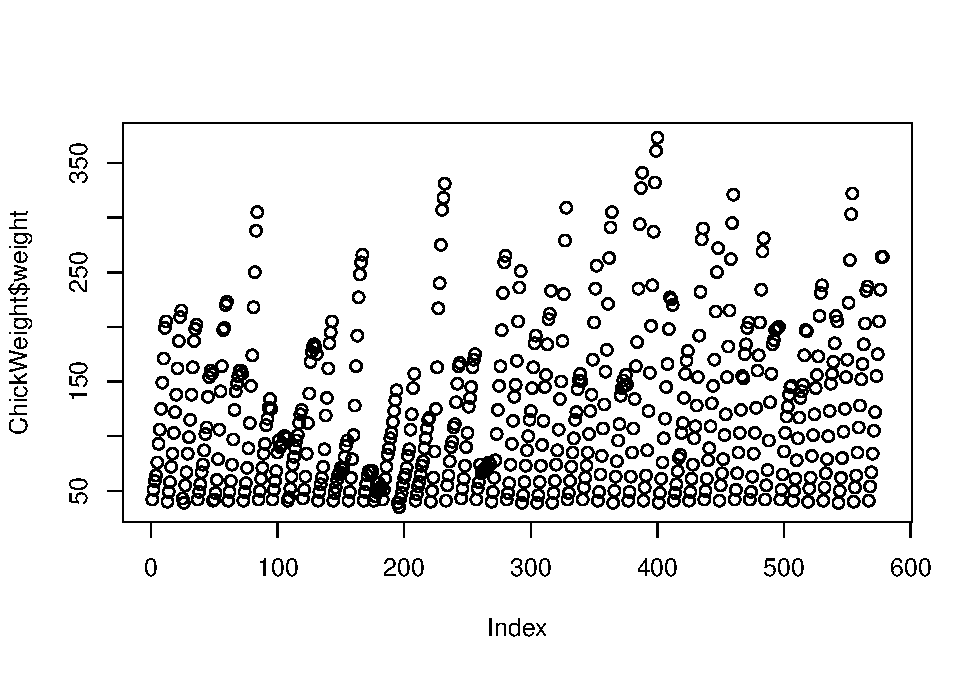
\includegraphics{01-intro_files/figure-latex/unnamed-chunk-5-1.pdf}

\begin{Shaded}
\begin{Highlighting}[]
\FunctionTok{plot}\NormalTok{(ChickWeight}\SpecialCharTok{$}\NormalTok{Diet, ChickWeight}\SpecialCharTok{$}\NormalTok{weight)}
\end{Highlighting}
\end{Shaded}

\includegraphics{01-intro_files/figure-latex/unnamed-chunk-6-1.pdf}

\begin{Shaded}
\begin{Highlighting}[]
\CommentTok{\# histogram}
\FunctionTok{hist}\NormalTok{(ChickWeight}\SpecialCharTok{$}\NormalTok{Deviation)}
\end{Highlighting}
\end{Shaded}

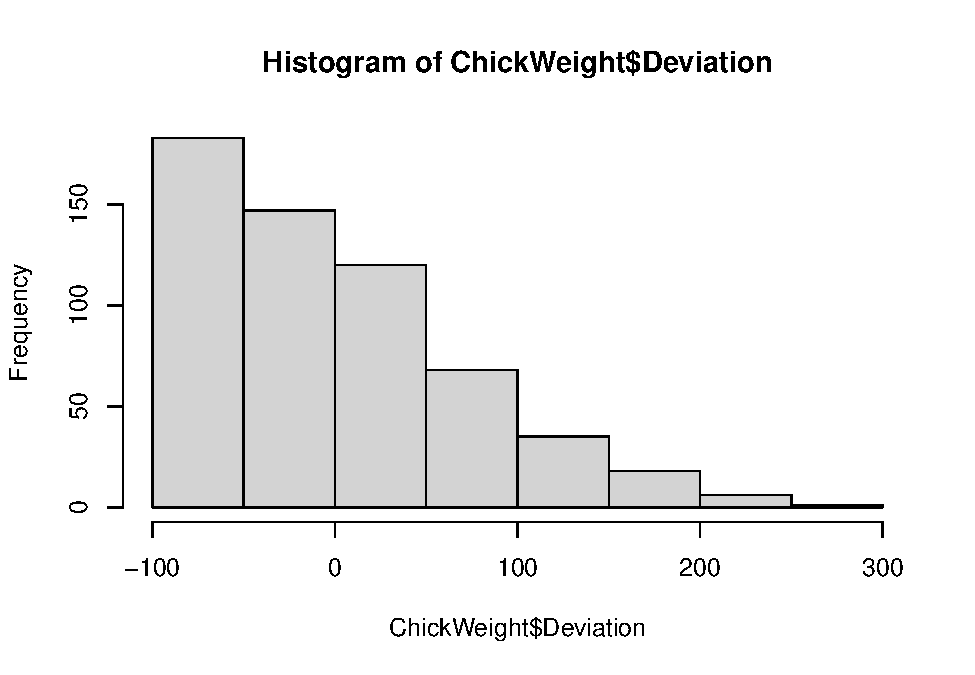
\includegraphics{01-intro_files/figure-latex/unnamed-chunk-7-1.pdf}

\hypertarget{tidyverse}{%
\chapter{Tidyverse}\label{tidyverse}}

The tidyverse has its own book called \emph{R for Data Science} by Hadley Wickham \& Garrett Grolemund (available online). This section will discuss a few functions out of the library that are very useful to know.

\hypertarget{tidy-data}{%
\section{Tidy Data}\label{tidy-data}}

Data Transformation and Introduction to \textbf{Tidyverse} library. This section is by \textbf{RLadies Freiburg} Divya Seernani.
Tidy data is data that has data or values for each column (variable) and each row (observation). The paradigm:
\texttt{import} -\textgreater{} \texttt{tidy} -\textgreater{} {[}Transform \textless-\textgreater{} Visualize \textless-\textgreater{} Model{]} -\textgreater{} Communicate

\hypertarget{dplyr-library}{%
\subsection{dplyr library}\label{dplyr-library}}

Inside the \textbf{tidyverse} library is the dplyr library which is helpful when creating new variables, renaming or reordering observations, selecting specific observations and calculating summary statistics among many other functions.

The dataset for this section will be the Indian Census (2011), dataset is available \href{https://github.com/nishusharma1608/India-Census-2011-Analysis/blob/master/india-districts-census-2011.csv}{here}. \emph{Remember to click on `raw' data format first to load in data, you should see white background and black text CSV data, copy the url link in order to read in the data}.

The tidyverse library brings along other libraries and when you load tidyverse you will a bunch of warnings in the console, these are no concern to you, basically telling you that one library hides another for function use. To turn off warnings in your Rmd file, inside the code chunk \{r\} set warning to false \texttt{\{r,\ warning=\ FALSE,\ message=\ FALSE\}}.

\begin{Shaded}
\begin{Highlighting}[]
\CommentTok{\# step 1 {-} install tidyverse library}
\CommentTok{\# install.packages(\textquotesingle{}tidyverse\textquotesingle{})  \# comment{-}out to run }
\FunctionTok{library}\NormalTok{(tidyverse)}

\CommentTok{\# read in the data}
\NormalTok{india\_census }\OtherTok{=} \FunctionTok{read.csv}\NormalTok{(}\StringTok{\textquotesingle{}https://raw.githubusercontent.com/nishusharma1608/India{-}Census{-}2011{-}Analysis/master/india{-}districts{-}census{-}2011.csv\textquotesingle{}}\NormalTok{)}
\end{Highlighting}
\end{Shaded}

\hypertarget{filter}{%
\subsubsection{filter}\label{filter}}

We now want to \textbf{filter} data only from Maharashtra and Gajarat, we will call the variable \texttt{WestStates}.

\begin{Shaded}
\begin{Highlighting}[]
\NormalTok{WestStates }\OtherTok{=} \FunctionTok{filter}\NormalTok{(india\_census, state.name }\SpecialCharTok{==} \StringTok{\textquotesingle{}Maharashtra\textquotesingle{}} \SpecialCharTok{|}\NormalTok{ State.name }\SpecialCharTok{==}\StringTok{\textquotesingle{}Gajarat\textquotesingle{}}\NormalTok{) }
\end{Highlighting}
\end{Shaded}

\hypertarget{arrange}{%
\subsubsection{arrange}\label{arrange}}

\textbf{Arrange} the west states in descending order (highest to lowest) by agricultural workers.

\begin{Shaded}
\begin{Highlighting}[]
\NormalTok{AgriDist}\OtherTok{\textless{}{-}} \FunctionTok{arrange}\NormalTok{(WestStates, Agricultural\_Workers)}
\NormalTok{AgriDistDes}\OtherTok{\textless{}{-}} \FunctionTok{arrange}\NormalTok{(WestStates, }\FunctionTok{desc}\NormalTok{(Agricultural\_Workers))}
\end{Highlighting}
\end{Shaded}

\hypertarget{mutate}{%
\subsubsection{mutate}\label{mutate}}

Using the \textbf{mutate} function to calculate the percentage of computers \& internet per households.

\begin{Shaded}
\begin{Highlighting}[]
\NormalTok{india\_census }\OtherTok{=} \FunctionTok{mutate}\NormalTok{(india\_census,}
                      \AttributeTok{Percent\_Internet =}\NormalTok{ Households\_with\_Internet }\SpecialCharTok{/}\NormalTok{ Households }\SpecialCharTok{*} \DecValTok{100}\NormalTok{,}
                      \AttributeTok{Percent\_Computer =}\NormalTok{ Households\_with\_Computer }\SpecialCharTok{/}\NormalTok{ Households }\SpecialCharTok{*} \DecValTok{100}
\NormalTok{                      )}
\end{Highlighting}
\end{Shaded}

\hypertarget{select}{%
\subsubsection{select}\label{select}}

Now that we have the percent of homes with internet, let us \textbf{select} the data on households with latrines and bathing facilities.

\begin{Shaded}
\begin{Highlighting}[]
\NormalTok{ModernHomes }\OtherTok{=} \FunctionTok{select}\NormalTok{(india\_census,}
\NormalTok{                     State.name, District.name, Households, Having\_bathing\_facility\_Total\_Households,}
\NormalTok{                  Having\_latrine\_facility\_within\_the\_premises\_Total\_Households)}

\CommentTok{\# and standardize the results}
\NormalTok{ModernHomes2 }\OtherTok{=} \FunctionTok{mutate}\NormalTok{(ModernHomes, }\AttributeTok{PercentToilet =}\NormalTok{ Having\_latrine\_facility\_within\_the\_premises\_Total\_Households }\SpecialCharTok{/}\NormalTok{ Households }\SpecialCharTok{*} \DecValTok{100}\NormalTok{,}
                     \AttributeTok{PercentBath =}\NormalTok{ Having\_bathing\_facility\_Total\_Households }\SpecialCharTok{/}\NormalTok{ Households }\SpecialCharTok{*} \DecValTok{100}\NormalTok{)}
\end{Highlighting}
\end{Shaded}

Visualize the data with the library ggplot, which comes attached (loaded) with tidyverse, but is good to load it anyway.

\begin{Shaded}
\begin{Highlighting}[]
\FunctionTok{library}\NormalTok{(ggplot2)}

\NormalTok{ModernHomesPlot }\OtherTok{\textless{}{-}} \FunctionTok{ggplot}\NormalTok{(ModernHomes2, }\FunctionTok{aes}\NormalTok{(}\AttributeTok{x=}\NormalTok{PercentToilet, }\AttributeTok{y=}\NormalTok{PercentBath)) }\SpecialCharTok{+} 
  \FunctionTok{geom\_point}\NormalTok{(}\FunctionTok{aes}\NormalTok{(}\AttributeTok{col=}\NormalTok{State.name, }\AttributeTok{size=}\NormalTok{Households)) }\SpecialCharTok{+} 
  \FunctionTok{geom\_smooth}\NormalTok{(}\AttributeTok{method=}\StringTok{"glm"}\NormalTok{, }\AttributeTok{se=}\NormalTok{T) }\SpecialCharTok{+} 
  \FunctionTok{labs}\NormalTok{(}\AttributeTok{subtitle=}\StringTok{"Toilets and Baths"}\NormalTok{, }
       \AttributeTok{y=}\StringTok{"Percentage with Bath"}\NormalTok{, }
       \AttributeTok{x=}\StringTok{"Percentage with Toilet"}\NormalTok{, }
       \AttributeTok{title=}\StringTok{"Scatterplot"}\NormalTok{, }
       \AttributeTok{caption =} \StringTok{"Indian Census 2011"}\NormalTok{)}

\FunctionTok{plot}\NormalTok{(ModernHomesPlot)}
\CommentTok{\#\textgreater{} \textasciigrave{}geom\_smooth()\textasciigrave{} using formula \textquotesingle{}y \textasciitilde{} x\textquotesingle{}}
\end{Highlighting}
\end{Shaded}

\includegraphics{02-tidyverse_files/figure-latex/unnamed-chunk-6-1.pdf}

Summary of literacy for all our data by state

\begin{Shaded}
\begin{Highlighting}[]
\FunctionTok{summarise}\NormalTok{(india\_census, }\AttributeTok{Percent\_Literate =} \FunctionTok{mean}\NormalTok{(Literate}\SpecialCharTok{/}\NormalTok{Population}\SpecialCharTok{*}\DecValTok{100}\NormalTok{) )}
\CommentTok{\#\textgreater{}   Percent\_Literate}
\CommentTok{\#\textgreater{} 1          62.4632}

\NormalTok{Literacy }\OtherTok{=} \FunctionTok{group\_by}\NormalTok{(india\_census, State.name)}

\NormalTok{LiteracyByState }\OtherTok{=} \FunctionTok{summarise}\NormalTok{(Literacy, }\AttributeTok{PercentLiterate =} \FunctionTok{mean}\NormalTok{(Literate}\SpecialCharTok{/}\NormalTok{Population}\SpecialCharTok{*}\DecValTok{100}\NormalTok{) )}
\end{Highlighting}
\end{Shaded}

An exercise example, literacy and toilets.

\begin{verbatim}
LiteracyHygiene <- select(india.districts.census.2011, State.name, District.name, Literate, Households, Having_latrine_facility_within_the_premises_Total_Households)
LiteracyHygiene_Calculated<-mutate(LiteracyHygiene, PercentToilet = Having_latrine_facility_within_the_premises_Total_Households / Households * 100,
                     AverageLiterate = Literate/Households)

LiteracyHygienePlot <- ggplot(LiteracyHygiene_Calculated, aes(x=PercentToilet, y=AverageLiterate)) + 
  geom_point(aes(col=State.name, size=Households)) + 
  geom_smooth(method="glm", se=T) + 
  labs(subtitle="Toilets and Baths", 
       y="Average Literate People per Household", 
       x="Percentage with Toilet", 
       title="Scatterplot", 
       caption = "Indian Census 2011")

plot(LiteracyHygienePlot)

library(plotly)
ggplotly(LiteracyHygienePlot)
\end{verbatim}

\hypertarget{geo-data}{%
\chapter{Geo Data}\label{geo-data}}

This section is all about geographical data and visualization.

\hypertarget{raster-and-vectors}{%
\section{raster and vectors}\label{raster-and-vectors}}

This tutorial is by \textbf{RLadies Freiburg} Elisa Schneider.
There are different ways to plot maps in R. The packages you use will depend on which your aim is and on the format of your data. Sometimes, geographical data can be simply in a \textbf{.txt or .csv file}, where you have one column for latitude and one for longitude and other variables or measurements corresponding to that location in the following columns. Yo can also have \textbf{shape files}, which are special files for geographical information. This files may contain points, lines or polygons. They are usually \textbf{.shp} files. Finally you can have \textbf{raster files} which are something similar to pictures or .png files because these files have pixels and (at least) a value associated with each pixel. The difference between a .png file and a shape file is that the shape-file has associated coordinates that locate this pixels on a specific surface of the world. The format is usually \textbf{.geotiff} or just \textbf{.tiff}.

In this meetup we will cover the basis of working with this formats. But this is only the starting point. There is a lot out there.

\hypertarget{simplest-example}{%
\subsection{Simplest example}\label{simplest-example}}

We can just use \texttt{geom\_polygon} from the library \texttt{ggplot} to create our first figure. Let´s suppose we know the latitude and the longitude of all the nodes in our polygon. How can we plot it?

\begin{verbatim}
require(ggplot2)
funny <- data.frame(lat = c(62, 55, 48, 48, 62), long = c(20,10.5,20,10,10)) # from top right 
#following the clock
ggplot(funny, aes(x = long, y = lat)) + # we specify the data
  geom_polygon(fill="green") + # we plot it
  geom_point(aes(x=13.25, y=50.5), color="violet", size=18) # we can also add points this was
\end{verbatim}

\hypertarget{information-already-availabe-in-r}{%
\subsection{Information already availabe in R}\label{information-already-availabe-in-r}}

The geometry of the polygons of the countries in the world are already loaded into R. You can access this info using the function \texttt{map\_data} from the package \texttt{ggplot2}.

How do we plot only one or a subset of countries?

We need to get the data for the geometry of the countries. To do that we use the library \texttt{maps} and \texttt{ggplot2}.

\begin{verbatim}
countries <- c("Germany", "France")
# Get the data
some.maps <- map_data("world", region = countries) # This function retrieves the data. The data we get is a df with lat and long of each node. 
head(some.maps)
require(dplyr)
require(tidyr)
# Mean of lat and long to then write the labels 
lab.data <- some.maps %>%
  group_by(region) %>%
  summarise(long = mean(long), lat = mean(lat))
lab.data
\end{verbatim}

\textbf{Themes in ggplot} In ggplot2 the display of non-data components is controlled by the theme system. The theme system of ggplot2 allows the manipulation of titles, labels, legends, grid lines and backgrounds. There are various build-in themes available that already have an all-around consistent style. A very common one for plotting data is \texttt{theme\_bw()} and \texttt{theme\_map()}. We use \texttt{theme\_map()} which will give our plot the appearance of a map. To use \texttt{theme\_map()} we need to load the package \texttt{ggthemes()}.

\begin{verbatim}
require(ggthemes)
fra_and_ger <- ggplot(some.maps, aes(x = long, y = lat)) +
  geom_polygon(aes( group = group, fill = region))+ #plot polygon, use group to group all the nodes of the same country together. 
  geom_text(aes(label = region), data = lab.data,  size = 3, hjust = 0.5)
#using theme_map
fra_and_ger + #print labels
  theme_map() +
  theme(legend.position = "none")
#Using theme bw
fra_and_ger + #print labels
  theme_bw() +
  theme(legend.position = "none")+
  xlab("Longitude") + ylab("Latitude")
 
\end{verbatim}

\hypertarget{the-world}{%
\subsection{the world}\label{the-world}}

From a couple of countries to the whole world: Plotting simple and nice maps of the world

\texttt{ggplot2} is becoming the standard for R graphs. However, it does not handle spatial data specifically. Handling spatial objects in R relies on Spatial classes defined in the package \texttt{sp} or \texttt{sf}. ggplot2 allows the use of spatial data through the package \texttt{sf}. \texttt{sf} elements can be added as layers in a graph. The combination of \texttt{ggplot2} and \texttt{sf} enables to create maps, using the grammar of graphics,but incorporation geographical info.

\hypertarget{we-can-just-create-a-map-from-the-world.}{%
\subsubsection{1. We can just create a map from the world.}\label{we-can-just-create-a-map-from-the-world.}}

We will do this using the library \texttt{ggplot2}.

The function \texttt{ne\_countries} also retrieves info about the countries. But now you do not get just nodes with coordinates but an \texttt{sf} object that contains much more info.

\begin{verbatim}
require(rnaturalearth)
require(rnaturalearthdata)
require(sf)
world <- ne_countries(scale = "medium", returnclass = "sf") # this is another function to get polygons of countries. 
class(world)
dim(world)
head(world[, 1:5])
\end{verbatim}

We can plot this geographical object using \texttt{ggplot2} and geometry \texttt{geom\_sf}

\begin{verbatim}
plot_w1 <- ggplot(data = world) +
    theme_bw()+ 
    geom_sf() + 
    xlab("Longitude") + ylab("Latitude") + 
    ggtitle("World map", subtitle = paste0("(", dim(world)[1], " countries)"))
plot_w1
\end{verbatim}

\hypertarget{we-can-change-the-colors-add-text}{%
\subsubsection{2. We can change the colors, add text \ldots{}}\label{we-can-change-the-colors-add-text}}

\begin{verbatim}
plot_w1 +
   geom_sf(color="blue", fill="black") +
  theme(panel.background = element_rect(fill = "black"))+# Modify the theme to change the background 
  #Where was the funny polygon located?
  geom_polygon(data=funny, aes(x = long, y = lat), color="green", fill="green") + # we plot it
  # Add points using lat-lon information
  geom_point(aes(x=13.25, y=50.5), color="violet", size=2)
\end{verbatim}

However our nice modern-art-style polygon looks different in the map compared to the first plot. \textbf{Any idea about what is happening?}

\hypertarget{coordinate-reference-systems-crs.}{%
\subsubsection{Coordinate reference systems (crs).}\label{coordinate-reference-systems-crs.}}

Going from the rear world (the earth) to the simplifyed model (the map)

\hypertarget{after-choosing-elipsoid-and-datum-we-have-to-project-from-3d-to-2d.}{%
\subsubsection{After choosing elipsoid and datum we have to project from 3D to 2D.}\label{after-choosing-elipsoid-and-datum-we-have-to-project-from-3d-to-2d.}}

You can get a feeling of how the Mercator projection distorts our worldview at \href{https://thetruesize.com}{link}.

Google and many apps use unprojected coordinates. When the coordinates are unprojected, they are in degrees and give the position on an sphere and not in a 2D surface. But, you still need an ellipsoid and datum to make clear which reference system you are using. All this information is coded in an \textbf{EPSG} code.
The most common coordinate reference system \textbf{crs} (used by Google and most apps) is EPGS: 4326. When you have lat Lon coordinates and no more info, it is likely that the EPSG is 4326, which uses the datum WGS84.

To get a taste:
\href{https://epsg.io/map\#srs=4326\&x=0.000000\&y=0.000000\&z=1\&layer=streets}{EPSG: 4326}
\href{https://epsg.io}{Coordinate Systems Worldwide}

To find the one used in your region of interest:

\href{https://spatialreference.org/ref/?search=argentina}{Argentina}
\href{https://spatialreference.org/ref/?search=germany}{Germany}
\href{https://spatialreference.org/ref/?search=europe}{Europe}

\hypertarget{make-choropleth-map}{%
\section{Make Choropleth Map}\label{make-choropleth-map}}

What is a \emph{Chorophlet Map}? ``A choropleth map is a thematic map in which areas are shaded or patterned in proportion to the measurement of the statistical variable being displayed on the map, such as population density or per-capita income.''(\href{https://en.Wikipedia.org/wiki/Choropleth_map}{Wikipedia})

\hypertarget{load-data}{%
\subsubsection{1. Load Data}\label{load-data}}

\begin{verbatim}
require(readr) # to use the function read_csv()
life.exp <- read_csv("data/LifeExp.csv")
\end{verbatim}

The data was obtained from \href{https://www.kaggle.com/kumarajarshi/life-expectancy-who}{link}, lot of cool data-sets are available for free.

\hypertarget{tidy-the-data-set}{%
\subsubsection{2. Tidy the data set}\label{tidy-the-data-set}}

have one column with country and another with life expectancy

\begin{verbatim}
life_exp <- life.exp %>%
  filter(year == 2016 & sex == "Both sexes") %>%  # Keep data for 2016 and for both sex
  dplyr::select(country, value) %>%                      # Select the two columns of interest
  rename(name = country, lifeExp = value) %>%   # Rename columns
  #We have a very common proble when using different sources, the name of the countries not allways match
  # Replace "United States of America" by USA in the region column
  mutate(
    name = ifelse(name == "United States of America", "United States", name), 
    name = ifelse(name == "Russian Federation", "Russia", name)
    )
\end{verbatim}

\hypertarget{get-data-of-the-polygons}{%
\subsubsection{3. Get data of the polygons}\label{get-data-of-the-polygons}}

of each country and merge map and life expectancy data

\begin{verbatim}
#attribute names
colnames(world)
life_exp2 <- left_join(world, life_exp, by = "name")
\end{verbatim}

\hypertarget{plot-with-ggpoligon}{%
\paragraph{4. Plot with ggpoligon}\label{plot-with-ggpoligon}}

\begin{verbatim}
life_exp_map <- ggplot(data = life_exp2) +
    geom_sf(aes(fill = lifeExp )) +
    scale_fill_viridis_c(option = "plasma", trans = "sqrt") # this allows you to choose different colour scale
life_exp_map
\end{verbatim}

Clearly we do not have information for all the countries regarding life expectancy and/or we have some problems with non-matching country names. When we call \texttt{left\_join} we only keep in the table the countries that are in the left table.

\hypertarget{add-points}{%
\subsubsection{5. Add points}\label{add-points}}

We can also add points to our plot. For example we could add some capitals. Points where samples were obtained, etc. We can also control the size and color of the points using another variable. For example, we could plot sample points and the size would be number of observations. We could plot one point per city and the size number of inhabitants\ldots and so son and so forth.

\begin{verbatim}
country_capitals <- read_csv("data/country-capitals.csv")
south_america_capitals <- country_capitals %>% dplyr::filter(ContinentName == "South America")
south_america_capitals$CapitalLatitude <- as.numeric(south_america_capitals$CapitalLatitude)
require(ggrepel)
life_exp_map +
  geom_point(data=south_america_capitals, 
             aes(x=CapitalLongitude, y=CapitalLatitude),
             alpha=0.5)+
  geom_text_repel(data=south_america_capitals, # geom_text_repel avoidsoverlapping
            aes( x=CapitalLongitude, y=CapitalLatitude, label=CapitalName), 
            hjust=0, vjust=0, size= 3)+ 
  theme_bw()
  
\end{verbatim}

\hypertarget{add-scale-and-north}{%
\subsubsection{6. Add scale and north}\label{add-scale-and-north}}

\begin{verbatim}
require(ggspatial)
life_exp_map + 
  annotation_scale(location = "bl", width_hint = 0.5) + # scale
    annotation_north_arrow(location = "bl", which_north = "true", #north arrow
        pad_x = unit(0.75, "in"), pad_y = unit(0.5, "in"),
        style = north_arrow_fancy_orienteering) +
    coord_sf(xlim = c(-20.15, 50.12), ylim = c(35.65, -45)) #crop
\end{verbatim}

\hypertarget{rasters-and-polygons}{%
\section{Rasters and polygons}\label{rasters-and-polygons}}

Usually spatial data comes as a \textbf{raster} or as a \textbf{polygon} format. We usually have shape files with the onformation of sampling sites, neighborhoods, streets, rivers, hospitals, surveys, etc. saved as .shp files.
Or we have lat-Lon data that we can transform into an sf object as we did before.
We can also get raster files such as climate raster files or remote sensing data, land use, etc. Most of the times we want to plot all this info together (raster + one or more shape-files).

\begin{verbatim}
require(rgdal)
require(raster) #Package to work with raster files
require(sf) #Package to work with shape files
\end{verbatim}

All this libraries allow us to work with spatial data using R.

\begin{itemize}
\item
  \texttt{rgdal} is a library that that allows us to read and write geospatial data in R. The library just translates the already existing library \texttt{gdal} into R. The link to \texttt{gdal}project is \href{https://gdal.org/}{link}.
\item
  \texttt{raster} is the library that we use to work with raster formats.
\item
  \texttt{sf} encodes spatial vector data. We already used it.
\end{itemize}

\hypertarget{load-the-raster-files-and-do-some-calculations}{%
\subsubsection{2. Load the raster files and do some calculations}\label{load-the-raster-files-and-do-some-calculations}}

Let´s suppose he have different sampling points in Germany. We are interested in the temperature difference between summer and winter in this sites. Can we do a map to display this info? How would you do that?

\hypertarget{this-are-some-usefull-links-to-find-data}{%
\subsubsection{This are some usefull links to find data:}\label{this-are-some-usefull-links-to-find-data}}

Link to the \href{https://www.bkg.bund.de/DE/Home/home.html}{Federal Agency for Cartography}
Link to \href{https://www.lgl-bw.de/lgl-internet/opencms/de/07_Produkte_und_Dienstleistungen/Open_Data_Initiative/}{open BW data}
Link to \href{http://worldclim.org/version2}{WoldClim}
link to \href{https://land.copernicus.eu/pan-european/corine-land-cover}{land use data}
Another useful \href{https://www.eea.europa.eu}{link}

All the data used in this example was download from this sites or directly from R.

All the data used in this example was download from this sites or directly from R.

\begin{verbatim}
t_july<-raster("data/wc2.0_5m_tavg_07.tif") # loads the raster
t_december<-raster("data/wc2.0_5m_tavg_01.tif") # loads the raster
# Get temperature range
t_diff <- abs(t_july - t_december)
plot(t_diff, main = "Temperature range")
\end{verbatim}

Raster calculation is relatively straight forward using R if the raster have the same resolution. If the raster come from different sources you usually have to re-shape one raster.

more info \href{https://rspatial.org/spatial/4-rasterdata.html}{here}

\hypertarget{load-the-shape-files}{%
\subsubsection{3. Load the shape files}\label{load-the-shape-files}}

\begin{verbatim}
sites<-st_read("data/sample_sites.shp") # loads the vector data - sites
#get germany voundaries from world R data
germany <- world %>%  dplyr::filter (name == "Germany")
plot(germany)
\end{verbatim}

As you can see here, each polling has associated data. Geometry has the info to build the polygon. \emph{level}, \emph{type}, etc. is the info related to each polygon. If the Polygons have different info in this fields, the polygons will be displayed in different colors.

\begin{verbatim}
#get germany voundaries from world R data
gfs <- world %>%  dplyr::filter (name %in% c("Germany", "Austria"))
plot(gfs)
\end{verbatim}

\hypertarget{check-reference-system}{%
\subsubsection{4. Check reference system}\label{check-reference-system}}

We have data coming from different sources, we have to check that the coordinate reference system match (otherwise we will have lots of problems and we will be doing everything wrong)

\begin{verbatim}
# The function to get the coor. system is different between shapes and rasters
st_crs(germany)#get the projection
st_crs(sites)#get the projection
crs(t_diff)#get the projection
st_crs(germany)$proj4string == st_crs(sites)$proj4string
st_crs(germany)$proj4string == crs(t_diff, asText = T)
\end{verbatim}

The data do not have the same coord. reference system. We have to transform one.

\begin{verbatim}
sites_transformed <- st_transform(sites, crs = crs(t_diff, asText = T))#transform coordinate sistem
germany_transformed <- st_transform(germany, crs = crs(t_diff, asText = T))#transform coordinate 
\end{verbatim}

\hypertarget{crop-the-raster-to-the-shape-file-extent}{%
\subsubsection{5. Crop the raster to the shape file extent}\label{crop-the-raster-to-the-shape-file-extent}}

We get the extent (the coordinates of the extreme points) for our shape file of Germany.

\begin{verbatim}
germany_extent <- extent(germany_transformed)
germany_extent
\end{verbatim}

\begin{verbatim}
# crop the land use data by the extend of BW. Crop funciton from the raster package
crop_tdiff <- crop(t_diff, germany_extent, snap = "out")
plot(crop_tdiff)
\end{verbatim}

In order to get a raster that matches exactly with the shape, we have to mask it.
We could also do this step without cropping first, but that would be much more computational intensive.

\begin{verbatim}
mask_tdiff <- mask(crop_tdiff, germany_transformed)
plot(mask_tdiff)
\end{verbatim}

\hypertarget{plot-with-tmap}{%
\subsubsection{\texorpdfstring{6. Plot with \texttt{tmap}}{6. Plot with tmap}}\label{plot-with-tmap}}

The library tmap is another grate option to build thematic maps. I find it very useful to work with raster data. Useful info can be found in the \href{https://cran.r-project.org/web/packages/tmap/vignettes/tmap-getstarted.html}{tmap vignette}. Another library to plot raster data is \texttt{rasterVis}. We will not cover it today but you can check the \href{https://oscarperpinan.github.io/rastervis/}{vignette}
You can plot many layers together. Each needs some reference(point, raster, text, etc.)

\begin{verbatim}
require(tmap)
tmap_mode("plot") # static plot or leaflet. 
tm_shape(mask_tdiff) + 
  tm_raster (col= "layer" , style = "cont", n=10,  title = "T. Difference") +
tm_shape(germany_transformed) + #add ploygon of germany
  tm_borders() +
tm_shape(sites_transformed) +
   tm_symbols(col = "gray", scale = .5)+ ##add points
      tm_text("Site", size = 0.8,  ymod=-0.6, root=1, size.lowerbound = .60, #add text
        bg.color="gray", bg.alpha = .5) +
tm_layout(inner.margins = c(0.15, 0.30, 0.10, 0.1)) + # crop the extent of the map
tm_layout(legend.position = c("left","bottom")) + # add legent
    tm_compass() + # add north
  tm_scale_bar() #add scale
\end{verbatim}

\begin{verbatim}
tm <- tm_shape(mask_tdiff) + 
  tm_raster (col= "layer" , style = "cont", n=10,  title = "T. Difference") +
tm_shape(germany_transformed) + #add ploygon of germany
  tm_borders() +
tm_shape(sites_transformed) +
   tm_symbols(col = "gray", scale = .5)+ ##add points
      tm_text("Site", size = 0.8,  ymod=-0.6, root=1, size.lowerbound = .60, #add text
        bg.color="gray", bg.alpha = .5) +
tm_layout(inner.margins = c(0.15, 0.30, 0.10, 0.1)) + # crop the extent of the map
tm_layout(legend.position = c("left","bottom")) + # add legent
    tm_compass() + # add north
  tm_scale_bar() #add scale
tmap_save(tm, filename = "t_range.png")
\end{verbatim}

With tmap is really easy to do interactive maps!

\begin{verbatim}
require(tmap)
tmap_mode("view")
tm_shape(mask_tdiff) +
  tm_raster (col= "layer" , style = "cont", n=10,  title = "T. Difference") +
tm_shape(germany_transformed) +
  tm_borders() +
tm_shape(sites_transformed) +
   tm_symbols(col = "gray", scale = .5)+
      tm_text("Site", size = 0.8,  ymod=-0.6, root=1, size.lowerbound = .60, 
        bg.color="gray", bg.alpha = .5) +
tm_layout(inner.margins = c(0.1, 0.30, 0.10, 0.1)) +
tm_layout(legend.position = c("left","bottom"))
##Reclasify values in the rasta flie. Reclasify function of raster file function
\end{verbatim}

\texttt{tmap} is a great library to make maps. Check the \href{https://cran.r-project.org/web/packages/tmap/vignettes/tmap-getstarted.html}{vignette}

\hypertarget{regression}{%
\chapter{Regression}\label{regression}}

\hypertarget{linear-regression-models}{%
\section{Linear Regression Models}\label{linear-regression-models}}

Linear Regression or Linear Model (LM) using happiness data from the World Health Organization, this section is brought to you by \textbf{RLadies Freiburg} Divya and Elisa. The happiness data can be found \href{https://raw.githubusercontent.com/rladies/meetup-presentations_freiburg/master/2019-10-Modelling\%201\%20-\%20LM\%2C\%20LMM\%20and\%20plots/Happiness_2016.csv}{here}.

\begin{tabular}{l|l|r|r|r|r|r|r|r|r|r|r|r}
\hline
Country & Region & Happiness.Rank & Happiness.Score & Lower.Confidence.Interval & Upper.Confidence.Interval & Economy..GDP.per.Capita. & Family & Health..Life.Expectancy. & Freedom & Trust..Government.Corruption. & Generosity & Dystopia.Residual\\
\hline
Denmark & Western Europe & 1 & 7.526 & 7.460 & 7.592 & 1.44178 & 1.16374 & 0.79504 & 0.57941 & 0.44453 & 0.36171 & 2.73939\\
\hline
Switzerland & Western Europe & 2 & 7.509 & 7.428 & 7.590 & 1.52733 & 1.14524 & 0.86303 & 0.58557 & 0.41203 & 0.28083 & 2.69463\\
\hline
Iceland & Western Europe & 3 & 7.501 & 7.333 & 7.669 & 1.42666 & 1.18326 & 0.86733 & 0.56624 & 0.14975 & 0.47678 & 2.83137\\
\hline
Norway & Western Europe & 4 & 7.498 & 7.421 & 7.575 & 1.57744 & 1.12690 & 0.79579 & 0.59609 & 0.35776 & 0.37895 & 2.66465\\
\hline
Finland & Western Europe & 5 & 7.413 & 7.351 & 7.475 & 1.40598 & 1.13464 & 0.81091 & 0.57104 & 0.41004 & 0.25492 & 2.82596\\
\hline
Canada & North America & 6 & 7.404 & 7.335 & 7.473 & 1.44015 & 1.09610 & 0.82760 & 0.57370 & 0.31329 & 0.44834 & 2.70485\\
\hline
\end{tabular}

The question is, \emph{what parameters are there? What questions can we address using these factors.?} \emph{Does trust in government a variable?}

\begin{Shaded}
\begin{Highlighting}[]
\FunctionTok{plot}\NormalTok{(happiness\_2016}\SpecialCharTok{$}\NormalTok{Happiness.Score, happiness\_2016}\SpecialCharTok{$}\NormalTok{Trust..Government.Corruption.)}
\end{Highlighting}
\end{Shaded}

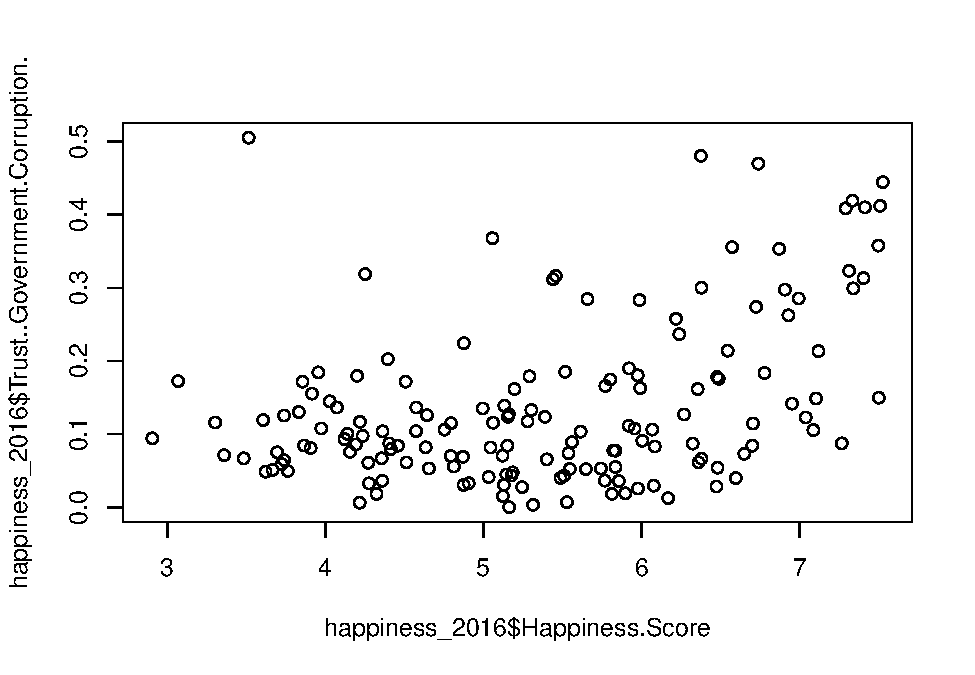
\includegraphics{04-regression_files/figure-latex/pressure-1.pdf}

\hypertarget{try-some-models}{%
\subsection{try some models}\label{try-some-models}}

There are 3 questions we could ask:
- Does Corruption within the government predict happiness of its citizens?
- How can we add Freedom as a predictor to the model?
- What is the difference between adding factors and looking at their interactions?

\begin{Shaded}
\begin{Highlighting}[]
\DocumentationTok{\#\# ANSWERS}
\CommentTok{\#fit our regression model}
\NormalTok{RegressionModel }\OtherTok{\textless{}{-}} \FunctionTok{lm}\NormalTok{(Happiness.Score }\SpecialCharTok{\textasciitilde{}}\NormalTok{ Trust..Government.Corruption., }\CommentTok{\# regression formula}
              \AttributeTok{data=}\NormalTok{happiness\_2016) }\CommentTok{\# data set}

\CommentTok{\# Summarize and print the results}
\FunctionTok{summary}\NormalTok{(RegressionModel) }\CommentTok{\# show regression coefficients table}
\CommentTok{\#\textgreater{} }
\CommentTok{\#\textgreater{} Call:}
\CommentTok{\#\textgreater{} lm(formula = Happiness.Score \textasciitilde{} Trust..Government.Corruption., }
\CommentTok{\#\textgreater{}     data = happiness\_2016)}
\CommentTok{\#\textgreater{} }
\CommentTok{\#\textgreater{} Residuals:}
\CommentTok{\#\textgreater{}     Min      1Q  Median      3Q     Max }
\CommentTok{\#\textgreater{} {-}3.3867 {-}0.7337  0.0653  0.8163  2.0929 }
\CommentTok{\#\textgreater{} }
\CommentTok{\#\textgreater{} Coefficients:}
\CommentTok{\#\textgreater{}                               Estimate Std. Error t value}
\CommentTok{\#\textgreater{} (Intercept)                     4.8133     0.1335  36.042}
\CommentTok{\#\textgreater{} Trust..Government.Corruption.   4.1336     0.7562   5.466}
\CommentTok{\#\textgreater{}                               Pr(\textgreater{}|t|)    }
\CommentTok{\#\textgreater{} (Intercept)                    \textless{} 2e{-}16 ***}
\CommentTok{\#\textgreater{} Trust..Government.Corruption.  1.8e{-}07 ***}
\CommentTok{\#\textgreater{} {-}{-}{-}}
\CommentTok{\#\textgreater{} Signif. codes:  }
\CommentTok{\#\textgreater{} 0 \textquotesingle{}***\textquotesingle{} 0.001 \textquotesingle{}**\textquotesingle{} 0.01 \textquotesingle{}*\textquotesingle{} 0.05 \textquotesingle{}.\textquotesingle{} 0.1 \textquotesingle{} \textquotesingle{} 1}
\CommentTok{\#\textgreater{} }
\CommentTok{\#\textgreater{} Residual standard error: 1.049 on 155 degrees of freedom}
\CommentTok{\#\textgreater{} Multiple R{-}squared:  0.1616, Adjusted R{-}squared:  0.1562 }
\CommentTok{\#\textgreater{} F{-}statistic: 29.88 on 1 and 155 DF,  p{-}value: 1.798e{-}07}


\NormalTok{RegressionModel2 }\OtherTok{\textless{}{-}} \FunctionTok{lm}\NormalTok{(Happiness.Score }\SpecialCharTok{\textasciitilde{}}\NormalTok{ Trust..Government.Corruption. }\SpecialCharTok{+}\NormalTok{ Freedom,}
                      \AttributeTok{data=}\NormalTok{happiness\_2016) }
\FunctionTok{summary}\NormalTok{(RegressionModel2) }
\CommentTok{\#\textgreater{} }
\CommentTok{\#\textgreater{} Call:}
\CommentTok{\#\textgreater{} lm(formula = Happiness.Score \textasciitilde{} Trust..Government.Corruption. + }
\CommentTok{\#\textgreater{}     Freedom, data = happiness\_2016)}
\CommentTok{\#\textgreater{} }
\CommentTok{\#\textgreater{} Residuals:}
\CommentTok{\#\textgreater{}      Min       1Q   Median       3Q      Max }
\CommentTok{\#\textgreater{} {-}3.12005 {-}0.75060  0.08456  0.70370  1.99165 }
\CommentTok{\#\textgreater{} }
\CommentTok{\#\textgreater{} Coefficients:}
\CommentTok{\#\textgreater{}                               Estimate Std. Error t value}
\CommentTok{\#\textgreater{} (Intercept)                     3.7395     0.2047  18.270}
\CommentTok{\#\textgreater{} Trust..Government.Corruption.   1.6146     0.7785   2.074}
\CommentTok{\#\textgreater{} Freedom                         3.8288     0.5940   6.445}
\CommentTok{\#\textgreater{}                               Pr(\textgreater{}|t|)    }
\CommentTok{\#\textgreater{} (Intercept)                    \textless{} 2e{-}16 ***}
\CommentTok{\#\textgreater{} Trust..Government.Corruption.   0.0397 *  }
\CommentTok{\#\textgreater{} Freedom                       1.41e{-}09 ***}
\CommentTok{\#\textgreater{} {-}{-}{-}}
\CommentTok{\#\textgreater{} Signif. codes:  }
\CommentTok{\#\textgreater{} 0 \textquotesingle{}***\textquotesingle{} 0.001 \textquotesingle{}**\textquotesingle{} 0.01 \textquotesingle{}*\textquotesingle{} 0.05 \textquotesingle{}.\textquotesingle{} 0.1 \textquotesingle{} \textquotesingle{} 1}
\CommentTok{\#\textgreater{} }
\CommentTok{\#\textgreater{} Residual standard error: 0.9337 on 154 degrees of freedom}
\CommentTok{\#\textgreater{} Multiple R{-}squared:  0.3397, Adjusted R{-}squared:  0.3312 }
\CommentTok{\#\textgreater{} F{-}statistic: 39.62 on 2 and 154 DF,  p{-}value: 1.313e{-}14}


\NormalTok{RegressionModel3 }\OtherTok{\textless{}{-}} \FunctionTok{lm}\NormalTok{(Happiness.Score }\SpecialCharTok{\textasciitilde{}}\NormalTok{ Trust..Government.Corruption. }\SpecialCharTok{*}\NormalTok{ Freedom, }
                       \AttributeTok{data=}\NormalTok{happiness\_2016) }

\FunctionTok{summary}\NormalTok{(RegressionModel3)}
\CommentTok{\#\textgreater{} }
\CommentTok{\#\textgreater{} Call:}
\CommentTok{\#\textgreater{} lm(formula = Happiness.Score \textasciitilde{} Trust..Government.Corruption. * }
\CommentTok{\#\textgreater{}     Freedom, data = happiness\_2016)}
\CommentTok{\#\textgreater{} }
\CommentTok{\#\textgreater{} Residuals:}
\CommentTok{\#\textgreater{}     Min      1Q  Median      3Q     Max }
\CommentTok{\#\textgreater{} {-}3.4328 {-}0.6808  0.1590  0.6513  2.0290 }
\CommentTok{\#\textgreater{} }
\CommentTok{\#\textgreater{} Coefficients:}
\CommentTok{\#\textgreater{}                                       Estimate Std. Error}
\CommentTok{\#\textgreater{} (Intercept)                             4.6015     0.3507}
\CommentTok{\#\textgreater{} Trust..Government.Corruption.          {-}7.0035     2.9817}
\CommentTok{\#\textgreater{} Freedom                                 1.8776     0.8728}
\CommentTok{\#\textgreater{} Trust..Government.Corruption.:Freedom  17.7259     5.9306}
\CommentTok{\#\textgreater{}                                       t value Pr(\textgreater{}|t|)    }
\CommentTok{\#\textgreater{} (Intercept)                            13.119  \textless{} 2e{-}16 ***}
\CommentTok{\#\textgreater{} Trust..Government.Corruption.          {-}2.349  0.02011 *  }
\CommentTok{\#\textgreater{} Freedom                                 2.151  0.03303 *  }
\CommentTok{\#\textgreater{} Trust..Government.Corruption.:Freedom   2.989  0.00326 ** }
\CommentTok{\#\textgreater{} {-}{-}{-}}
\CommentTok{\#\textgreater{} Signif. codes:  }
\CommentTok{\#\textgreater{} 0 \textquotesingle{}***\textquotesingle{} 0.001 \textquotesingle{}**\textquotesingle{} 0.01 \textquotesingle{}*\textquotesingle{} 0.05 \textquotesingle{}.\textquotesingle{} 0.1 \textquotesingle{} \textquotesingle{} 1}
\CommentTok{\#\textgreater{} }
\CommentTok{\#\textgreater{} Residual standard error: 0.9105 on 153 degrees of freedom}
\CommentTok{\#\textgreater{} Multiple R{-}squared:  0.3762, Adjusted R{-}squared:  0.3639 }
\CommentTok{\#\textgreater{} F{-}statistic: 30.75 on 3 and 153 DF,  p{-}value: 1.293e{-}15}
\end{Highlighting}
\end{Shaded}

There are a number of different Parametric and non-parametric tests we can try in the same format. Instead of lm, we could use t.test(), aov(), wilcox.test(), kruskal.test().

Is there a categorical variable we can use to run an ANOVA on?

\emph{How does the happiness quotient differ based on regions?}

\begin{Shaded}
\begin{Highlighting}[]
\NormalTok{ANOVA }\OtherTok{\textless{}{-}} \FunctionTok{aov}\NormalTok{(Happiness.Score }\SpecialCharTok{\textasciitilde{}}\NormalTok{ Region, }
             \AttributeTok{data=}\NormalTok{happiness\_2016) }
\FunctionTok{summary}\NormalTok{(ANOVA) }
\CommentTok{\#\textgreater{}              Df Sum Sq Mean Sq F value Pr(\textgreater{}F)    }
\CommentTok{\#\textgreater{} Region        9 126.69  14.077      27 \textless{}2e{-}16 ***}
\CommentTok{\#\textgreater{} Residuals   147  76.64   0.521                   }
\CommentTok{\#\textgreater{} {-}{-}{-}}
\CommentTok{\#\textgreater{} Signif. codes:  }
\CommentTok{\#\textgreater{} 0 \textquotesingle{}***\textquotesingle{} 0.001 \textquotesingle{}**\textquotesingle{} 0.01 \textquotesingle{}*\textquotesingle{} 0.05 \textquotesingle{}.\textquotesingle{} 0.1 \textquotesingle{} \textquotesingle{} 1}
\FunctionTok{TukeyHSD}\NormalTok{(ANOVA)}
\CommentTok{\#\textgreater{}   Tukey multiple comparisons of means}
\CommentTok{\#\textgreater{}     95\% family{-}wise confidence level}
\CommentTok{\#\textgreater{} }
\CommentTok{\#\textgreater{} Fit: aov(formula = Happiness.Score \textasciitilde{} Region, data = happiness\_2016)}
\CommentTok{\#\textgreater{} }
\CommentTok{\#\textgreater{} $Region}
\CommentTok{\#\textgreater{}                                                                    diff}
\CommentTok{\#\textgreater{} Central and Eastern Europe{-}Australia and New Zealand        {-}1.95281034}
\CommentTok{\#\textgreater{} Eastern Asia{-}Australia and New Zealand                      {-}1.69933333}
\CommentTok{\#\textgreater{} Latin America and Caribbean{-}Australia and New Zealand       {-}1.22175000}
\CommentTok{\#\textgreater{} Middle East and Northern Africa{-}Australia and New Zealand   {-}1.93744737}
\CommentTok{\#\textgreater{} North America{-}Australia and New Zealand                     {-}0.06950000}
\CommentTok{\#\textgreater{} Southeastern Asia{-}Australia and New Zealand                 {-}1.98461111}
\CommentTok{\#\textgreater{} Southern Asia{-}Australia and New Zealand                     {-}2.76021429}
\CommentTok{\#\textgreater{} Sub{-}Saharan Africa{-}Australia and New Zealand                {-}3.18707895}
\CommentTok{\#\textgreater{} Western Europe{-}Australia and New Zealand                    {-}0.63783333}
\CommentTok{\#\textgreater{} Eastern Asia{-}Central and Eastern Europe                      0.25347701}
\CommentTok{\#\textgreater{} Latin America and Caribbean{-}Central and Eastern Europe       0.73106034}
\CommentTok{\#\textgreater{} Middle East and Northern Africa{-}Central and Eastern Europe   0.01536298}
\CommentTok{\#\textgreater{} North America{-}Central and Eastern Europe                     1.88331034}
\CommentTok{\#\textgreater{} Southeastern Asia{-}Central and Eastern Europe                {-}0.03180077}
\CommentTok{\#\textgreater{} Southern Asia{-}Central and Eastern Europe                    {-}0.80740394}
\CommentTok{\#\textgreater{} Sub{-}Saharan Africa{-}Central and Eastern Europe               {-}1.23426860}
\CommentTok{\#\textgreater{} Western Europe{-}Central and Eastern Europe                    1.31497701}
\CommentTok{\#\textgreater{} Latin America and Caribbean{-}Eastern Asia                     0.47758333}
\CommentTok{\#\textgreater{} Middle East and Northern Africa{-}Eastern Asia                {-}0.23811404}
\CommentTok{\#\textgreater{} North America{-}Eastern Asia                                   1.62983333}
\CommentTok{\#\textgreater{} Southeastern Asia{-}Eastern Asia                              {-}0.28527778}
\CommentTok{\#\textgreater{} Southern Asia{-}Eastern Asia                                  {-}1.06088095}
\CommentTok{\#\textgreater{} Sub{-}Saharan Africa{-}Eastern Asia                             {-}1.48774561}
\CommentTok{\#\textgreater{} Western Europe{-}Eastern Asia                                  1.06150000}
\CommentTok{\#\textgreater{} Middle East and Northern Africa{-}Latin America and Caribbean {-}0.71569737}
\CommentTok{\#\textgreater{} North America{-}Latin America and Caribbean                    1.15225000}
\CommentTok{\#\textgreater{} Southeastern Asia{-}Latin America and Caribbean               {-}0.76286111}
\CommentTok{\#\textgreater{} Southern Asia{-}Latin America and Caribbean                   {-}1.53846429}
\CommentTok{\#\textgreater{} Sub{-}Saharan Africa{-}Latin America and Caribbean              {-}1.96532895}
\CommentTok{\#\textgreater{} Western Europe{-}Latin America and Caribbean                   0.58391667}
\CommentTok{\#\textgreater{} North America{-}Middle East and Northern Africa                1.86794737}
\CommentTok{\#\textgreater{} Southeastern Asia{-}Middle East and Northern Africa           {-}0.04716374}
\CommentTok{\#\textgreater{} Southern Asia{-}Middle East and Northern Africa               {-}0.82276692}
\CommentTok{\#\textgreater{} Sub{-}Saharan Africa{-}Middle East and Northern Africa          {-}1.24963158}
\CommentTok{\#\textgreater{} Western Europe{-}Middle East and Northern Africa               1.29961404}
\CommentTok{\#\textgreater{} Southeastern Asia{-}North America                             {-}1.91511111}
\CommentTok{\#\textgreater{} Southern Asia{-}North America                                 {-}2.69071429}
\CommentTok{\#\textgreater{} Sub{-}Saharan Africa{-}North America                            {-}3.11757895}
\CommentTok{\#\textgreater{} Western Europe{-}North America                                {-}0.56833333}
\CommentTok{\#\textgreater{} Southern Asia{-}Southeastern Asia                             {-}0.77560317}
\CommentTok{\#\textgreater{} Sub{-}Saharan Africa{-}Southeastern Asia                        {-}1.20246784}
\CommentTok{\#\textgreater{} Western Europe{-}Southeastern Asia                             1.34677778}
\CommentTok{\#\textgreater{} Sub{-}Saharan Africa{-}Southern Asia                            {-}0.42686466}
\CommentTok{\#\textgreater{} Western Europe{-}Southern Asia                                 2.12238095}
\CommentTok{\#\textgreater{} Western Europe{-}Sub{-}Saharan Africa                            2.54924561}
\CommentTok{\#\textgreater{}                                                                     lwr}
\CommentTok{\#\textgreater{} Central and Eastern Europe{-}Australia and New Zealand        {-}3.64886668}
\CommentTok{\#\textgreater{} Eastern Asia{-}Australia and New Zealand                      {-}3.59354189}
\CommentTok{\#\textgreater{} Latin America and Caribbean{-}Australia and New Zealand       {-}2.92916652}
\CommentTok{\#\textgreater{} Middle East and Northern Africa{-}Australia and New Zealand   {-}3.66205885}
\CommentTok{\#\textgreater{} North America{-}Australia and New Zealand                     {-}2.38942221}
\CommentTok{\#\textgreater{} Southeastern Asia{-}Australia and New Zealand                 {-}3.79817773}
\CommentTok{\#\textgreater{} Southern Asia{-}Australia and New Zealand                     {-}4.62029016}
\CommentTok{\#\textgreater{} Sub{-}Saharan Africa{-}Australia and New Zealand                {-}4.87012741}
\CommentTok{\#\textgreater{} Western Europe{-}Australia and New Zealand                    {-}2.35460563}
\CommentTok{\#\textgreater{} Eastern Asia{-}Central and Eastern Europe                     {-}0.78700079}
\CommentTok{\#\textgreater{} Latin America and Caribbean{-}Central and Eastern Europe       0.09087351}
\CommentTok{\#\textgreater{} Middle East and Northern Africa{-}Central and Eastern Europe  {-}0.66936527}
\CommentTok{\#\textgreater{} North America{-}Central and Eastern Europe                     0.18725401}
\CommentTok{\#\textgreater{} Southeastern Asia{-}Central and Eastern Europe                {-}0.91700803}
\CommentTok{\#\textgreater{} Southern Asia{-}Central and Eastern Europe                    {-}1.78436365}
\CommentTok{\#\textgreater{} Sub{-}Saharan Africa{-}Central and Eastern Europe               {-}1.80630021}
\CommentTok{\#\textgreater{} Western Europe{-}Central and Eastern Europe                    0.65024012}
\CommentTok{\#\textgreater{} Latin America and Caribbean{-}Eastern Asia                    {-}0.58131144}
\CommentTok{\#\textgreater{} Middle East and Northern Africa{-}Eastern Asia                {-}1.32451715}
\CommentTok{\#\textgreater{} North America{-}Eastern Asia                                  {-}0.26437522}
\CommentTok{\#\textgreater{} Southeastern Asia{-}Eastern Asia                              {-}1.50798414}
\CommentTok{\#\textgreater{} Southern Asia{-}Eastern Asia                                  {-}2.35156652}
\CommentTok{\#\textgreater{} Sub{-}Saharan Africa{-}Eastern Asia                             {-}2.50688207}
\CommentTok{\#\textgreater{} Western Europe{-}Eastern Asia                                 {-}0.01241531}
\CommentTok{\#\textgreater{} Middle East and Northern Africa{-}Latin America and Caribbean {-}1.42809953}
\CommentTok{\#\textgreater{} North America{-}Latin America and Caribbean                   {-}0.55516652}
\CommentTok{\#\textgreater{} Southeastern Asia{-}Latin America and Caribbean               {-}1.66964442}
\CommentTok{\#\textgreater{} Southern Asia{-}Latin America and Caribbean                   {-}2.53501551}
\CommentTok{\#\textgreater{} Sub{-}Saharan Africa{-}Latin America and Caribbean              {-}2.57021260}
\CommentTok{\#\textgreater{} Western Europe{-}Latin America and Caribbean                  {-}0.10929268}
\CommentTok{\#\textgreater{} North America{-}Middle East and Northern Africa                0.14333589}
\CommentTok{\#\textgreater{} Southeastern Asia{-}Middle East and Northern Africa           {-}0.98592333}
\CommentTok{\#\textgreater{} Southern Asia{-}Middle East and Northern Africa               {-}1.84849980}
\CommentTok{\#\textgreater{} Sub{-}Saharan Africa{-}Middle East and Northern Africa          {-}1.90147345}
\CommentTok{\#\textgreater{} Western Europe{-}Middle East and Northern Africa               0.56507146}
\CommentTok{\#\textgreater{} Southeastern Asia{-}North America                             {-}3.72867773}
\CommentTok{\#\textgreater{} Southern Asia{-}North America                                 {-}4.55079016}
\CommentTok{\#\textgreater{} Sub{-}Saharan Africa{-}North America                            {-}4.80062741}
\CommentTok{\#\textgreater{} Western Europe{-}North America                                {-}2.28510563}
\CommentTok{\#\textgreater{} Southern Asia{-}Southeastern Asia                             {-}1.94473408}
\CommentTok{\#\textgreater{} Sub{-}Saharan Africa{-}Southeastern Asia                        {-}2.06248932}
\CommentTok{\#\textgreater{} Western Europe{-}Southeastern Asia                             0.42249865}
\CommentTok{\#\textgreater{} Sub{-}Saharan Africa{-}Southern Asia                            {-}1.38106345}
\CommentTok{\#\textgreater{} Western Europe{-}Southern Asia                                 1.10988389}
\CommentTok{\#\textgreater{} Western Europe{-}Sub{-}Saharan Africa                            1.91843647}
\CommentTok{\#\textgreater{}                                                                      upr}
\CommentTok{\#\textgreater{} Central and Eastern Europe{-}Australia and New Zealand        {-}0.256754011}
\CommentTok{\#\textgreater{} Eastern Asia{-}Australia and New Zealand                       0.194875220}
\CommentTok{\#\textgreater{} Latin America and Caribbean{-}Australia and New Zealand        0.485666516}
\CommentTok{\#\textgreater{} Middle East and Northern Africa{-}Australia and New Zealand   {-}0.212835891}
\CommentTok{\#\textgreater{} North America{-}Australia and New Zealand                      2.250422211}
\CommentTok{\#\textgreater{} Southeastern Asia{-}Australia and New Zealand                 {-}0.171044494}
\CommentTok{\#\textgreater{} Southern Asia{-}Australia and New Zealand                     {-}0.900138412}
\CommentTok{\#\textgreater{} Sub{-}Saharan Africa{-}Australia and New Zealand                {-}1.504030481}
\CommentTok{\#\textgreater{} Western Europe{-}Australia and New Zealand                     1.078938960}
\CommentTok{\#\textgreater{} Eastern Asia{-}Central and Eastern Europe                      1.293954817}
\CommentTok{\#\textgreater{} Latin America and Caribbean{-}Central and Eastern Europe       1.371247178}
\CommentTok{\#\textgreater{} Middle East and Northern Africa{-}Central and Eastern Europe   0.700091220}
\CommentTok{\#\textgreater{} North America{-}Central and Eastern Europe                     3.579366678}
\CommentTok{\#\textgreater{} Southeastern Asia{-}Central and Eastern Europe                 0.853406494}
\CommentTok{\#\textgreater{} Southern Asia{-}Central and Eastern Europe                     0.169555770}
\CommentTok{\#\textgreater{} Sub{-}Saharan Africa{-}Central and Eastern Europe               {-}0.662236994}
\CommentTok{\#\textgreater{} Western Europe{-}Central and Eastern Europe                    1.979713898}
\CommentTok{\#\textgreater{} Latin America and Caribbean{-}Eastern Asia                     1.536478105}
\CommentTok{\#\textgreater{} Middle East and Northern Africa{-}Eastern Asia                 0.848289078}
\CommentTok{\#\textgreater{} North America{-}Eastern Asia                                   3.524041887}
\CommentTok{\#\textgreater{} Southeastern Asia{-}Eastern Asia                               0.937428586}
\CommentTok{\#\textgreater{} Southern Asia{-}Eastern Asia                                   0.229804615}
\CommentTok{\#\textgreater{} Sub{-}Saharan Africa{-}Eastern Asia                             {-}0.468609157}
\CommentTok{\#\textgreater{} Western Europe{-}Eastern Asia                                  2.135415306}
\CommentTok{\#\textgreater{} Middle East and Northern Africa{-}Latin America and Caribbean {-}0.003295206}
\CommentTok{\#\textgreater{} North America{-}Latin America and Caribbean                    2.859666516}
\CommentTok{\#\textgreater{} Southeastern Asia{-}Latin America and Caribbean                0.143922197}
\CommentTok{\#\textgreater{} Southern Asia{-}Latin America and Caribbean                   {-}0.541913057}
\CommentTok{\#\textgreater{} Sub{-}Saharan Africa{-}Latin America and Caribbean              {-}1.360445294}
\CommentTok{\#\textgreater{} Western Europe{-}Latin America and Caribbean                   1.277126016}
\CommentTok{\#\textgreater{} North America{-}Middle East and Northern Africa                3.592558845}
\CommentTok{\#\textgreater{} Southeastern Asia{-}Middle East and Northern Africa            0.891595840}
\CommentTok{\#\textgreater{} Southern Asia{-}Middle East and Northern Africa                0.202965961}
\CommentTok{\#\textgreater{} Sub{-}Saharan Africa{-}Middle East and Northern Africa          {-}0.597789711}
\CommentTok{\#\textgreater{} Western Europe{-}Middle East and Northern Africa               2.034156606}
\CommentTok{\#\textgreater{} Southeastern Asia{-}North America                             {-}0.101544494}
\CommentTok{\#\textgreater{} Southern Asia{-}North America                                 {-}0.830638412}
\CommentTok{\#\textgreater{} Sub{-}Saharan Africa{-}North America                            {-}1.434530481}
\CommentTok{\#\textgreater{} Western Europe{-}North America                                 1.148438960}
\CommentTok{\#\textgreater{} Southern Asia{-}Southeastern Asia                              0.393527727}
\CommentTok{\#\textgreater{} Sub{-}Saharan Africa{-}Southeastern Asia                        {-}0.342446355}
\CommentTok{\#\textgreater{} Western Europe{-}Southeastern Asia                             2.271056910}
\CommentTok{\#\textgreater{} Sub{-}Saharan Africa{-}Southern Asia                             0.527334128}
\CommentTok{\#\textgreater{} Western Europe{-}Southern Asia                                 3.134878013}
\CommentTok{\#\textgreater{} Western Europe{-}Sub{-}Saharan Africa                            3.180054762}
\CommentTok{\#\textgreater{}                                                                 p adj}
\CommentTok{\#\textgreater{} Central and Eastern Europe{-}Australia and New Zealand        0.0110279}
\CommentTok{\#\textgreater{} Eastern Asia{-}Australia and New Zealand                      0.1200475}
\CommentTok{\#\textgreater{} Latin America and Caribbean{-}Australia and New Zealand       0.3959950}
\CommentTok{\#\textgreater{} Middle East and Northern Africa{-}Australia and New Zealand   0.0148505}
\CommentTok{\#\textgreater{} North America{-}Australia and New Zealand                     1.0000000}
\CommentTok{\#\textgreater{} Southeastern Asia{-}Australia and New Zealand                 0.0200680}
\CommentTok{\#\textgreater{} Southern Asia{-}Australia and New Zealand                     0.0001878}
\CommentTok{\#\textgreater{} Sub{-}Saharan Africa{-}Australia and New Zealand                0.0000004}
\CommentTok{\#\textgreater{} Western Europe{-}Australia and New Zealand                    0.9722986}
\CommentTok{\#\textgreater{} Eastern Asia{-}Central and Eastern Europe                     0.9987321}
\CommentTok{\#\textgreater{} Latin America and Caribbean{-}Central and Eastern Europe      0.0122030}
\CommentTok{\#\textgreater{} Middle East and Northern Africa{-}Central and Eastern Europe  1.0000000}
\CommentTok{\#\textgreater{} North America{-}Central and Eastern Europe                    0.0170083}
\CommentTok{\#\textgreater{} Southeastern Asia{-}Central and Eastern Europe                1.0000000}
\CommentTok{\#\textgreater{} Southern Asia{-}Central and Eastern Europe                    0.2021961}
\CommentTok{\#\textgreater{} Sub{-}Saharan Africa{-}Central and Eastern Europe               0.0000000}
\CommentTok{\#\textgreater{} Western Europe{-}Central and Eastern Europe                   0.0000001}
\CommentTok{\#\textgreater{} Latin America and Caribbean{-}Eastern Asia                    0.9092820}
\CommentTok{\#\textgreater{} Middle East and Northern Africa{-}Eastern Asia                0.9994553}
\CommentTok{\#\textgreater{} North America{-}Eastern Asia                                  0.1587204}
\CommentTok{\#\textgreater{} Southeastern Asia{-}Eastern Asia                              0.9990999}
\CommentTok{\#\textgreater{} Southern Asia{-}Eastern Asia                                  0.2085183}
\CommentTok{\#\textgreater{} Sub{-}Saharan Africa{-}Eastern Asia                             0.0002599}
\CommentTok{\#\textgreater{} Western Europe{-}Eastern Asia                                 0.0555311}
\CommentTok{\#\textgreater{} Middle East and Northern Africa{-}Latin America and Caribbean 0.0479233}
\CommentTok{\#\textgreater{} North America{-}Latin America and Caribbean                   0.4832340}
\CommentTok{\#\textgreater{} Southeastern Asia{-}Latin America and Caribbean               0.1822793}
\CommentTok{\#\textgreater{} Southern Asia{-}Latin America and Caribbean                   0.0000824}
\CommentTok{\#\textgreater{} Sub{-}Saharan Africa{-}Latin America and Caribbean              0.0000000}
\CommentTok{\#\textgreater{} Western Europe{-}Latin America and Caribbean                  0.1809182}
\CommentTok{\#\textgreater{} North America{-}Middle East and Northern Africa               0.0224810}
\CommentTok{\#\textgreater{} Southeastern Asia{-}Middle East and Northern Africa           1.0000000}
\CommentTok{\#\textgreater{} Southern Asia{-}Middle East and Northern Africa               0.2380242}
\CommentTok{\#\textgreater{} Sub{-}Saharan Africa{-}Middle East and Northern Africa          0.0000003}
\CommentTok{\#\textgreater{} Western Europe{-}Middle East and Northern Africa              0.0000030}
\CommentTok{\#\textgreater{} Southeastern Asia{-}North America                             0.0294290}
\CommentTok{\#\textgreater{} Southern Asia{-}North America                                 0.0003101}
\CommentTok{\#\textgreater{} Sub{-}Saharan Africa{-}North America                            0.0000008}
\CommentTok{\#\textgreater{} Western Europe{-}North America                                0.9873720}
\CommentTok{\#\textgreater{} Southern Asia{-}Southeastern Asia                             0.5086390}
\CommentTok{\#\textgreater{} Sub{-}Saharan Africa{-}Southeastern Asia                        0.0005847}
\CommentTok{\#\textgreater{} Western Europe{-}Southeastern Asia                            0.0002694}
\CommentTok{\#\textgreater{} Sub{-}Saharan Africa{-}Southern Asia                            0.9133646}
\CommentTok{\#\textgreater{} Western Europe{-}Southern Asia                                0.0000000}
\CommentTok{\#\textgreater{} Western Europe{-}Sub{-}Saharan Africa                           0.0000000}
\end{Highlighting}
\end{Shaded}

\hypertarget{independence-of-the-data}{%
\subsection{independence of the data}\label{independence-of-the-data}}

Let's think about the data and pose some questions.

\begin{enumerate}
\def\labelenumi{\Alph{enumi})}
\tightlist
\item
  Do you think that countries in the same region tend to be more similar to each other?
  If your answer is yes, then the countries are not really independent and identically distributed data. This could be a problem with statistical models. So you have three options:
\end{enumerate}

\begin{itemize}
\item
  \begin{enumerate}
  \def\labelenumi{\arabic{enumi}.}
  \tightlist
  \item
    Ignore the problem, or argue why you think your data IS independent (you will no be the only one)
  \end{enumerate}
\item
  \begin{enumerate}
  \def\labelenumi{\arabic{enumi}.}
  \setcounter{enumi}{1}
  \tightlist
  \item
    Do not ignore it, take the average of each region and then make a model using this average. Yes, what you think is correct, you loose a lot of data!
  \end{enumerate}
\item
  \begin{enumerate}
  \def\labelenumi{\arabic{enumi}.}
  \setcounter{enumi}{2}
  \tightlist
  \item
    Do one linear model for each region\ldots data costly (e.g.~Australia and North America have only two data points)
  \end{enumerate}
\item
  \begin{enumerate}
  \def\labelenumi{\arabic{enumi}.}
  \setcounter{enumi}{3}
  \tightlist
  \item
    Try a linear mixed model
  \end{enumerate}
\end{itemize}

\begin{enumerate}
\def\labelenumi{\Alph{enumi})}
\setcounter{enumi}{1}
\item
  How variable is the happiness between regions?
\item
  How does happiness depend on other predictors such as health, economy and generosity?
\end{enumerate}

\hypertarget{visualization-of-the-data}{%
\subsection{visualization of the data}\label{visualization-of-the-data}}

We can do some plots to see how data look like.
In this plot we visualize how economy affects happiness in every region. We could do one plot per predictor.

\begin{Shaded}
\begin{Highlighting}[]
\FunctionTok{library}\NormalTok{(dplyr)}
\CommentTok{\#\textgreater{} }
\CommentTok{\#\textgreater{} Attaching package: \textquotesingle{}dplyr\textquotesingle{}}
\CommentTok{\#\textgreater{} The following objects are masked from \textquotesingle{}package:stats\textquotesingle{}:}
\CommentTok{\#\textgreater{} }
\CommentTok{\#\textgreater{}     filter, lag}
\CommentTok{\#\textgreater{} The following objects are masked from \textquotesingle{}package:base\textquotesingle{}:}
\CommentTok{\#\textgreater{} }
\CommentTok{\#\textgreater{}     intersect, setdiff, setequal, union}
\FunctionTok{library}\NormalTok{(tidyr)}
\NormalTok{Happiness\_2016 }\OtherTok{\textless{}{-}}\NormalTok{ happiness\_2016 }\SpecialCharTok{\%\textgreater{}\%} \FunctionTok{group\_by}\NormalTok{(Region) }\SpecialCharTok{\%\textgreater{}\%} \FunctionTok{mutate}\NormalTok{(}\AttributeTok{mean.reg =} \FunctionTok{mean}\NormalTok{(Happiness.Score)) }\SpecialCharTok{\%\textgreater{}\%}  \FunctionTok{ungroup}\NormalTok{()}
\FunctionTok{library}\NormalTok{(ggplot2)}
\FunctionTok{ggplot}\NormalTok{(Happiness\_2016) }\SpecialCharTok{+} 
  \FunctionTok{aes}\NormalTok{(}\AttributeTok{x =}\NormalTok{ Economy..GDP.per.Capita., }\AttributeTok{y =}\NormalTok{ Happiness.Score) }\SpecialCharTok{+} 
  \FunctionTok{stat\_smooth}\NormalTok{(}\AttributeTok{method =} \StringTok{"lm"}\NormalTok{, }\AttributeTok{se =} \ConstantTok{FALSE}\NormalTok{) }\SpecialCharTok{+}
  \CommentTok{\# Put the points on top of lines}
  \FunctionTok{geom\_point}\NormalTok{() }\SpecialCharTok{+}
  \FunctionTok{facet\_wrap}\NormalTok{(}\StringTok{"Region"}\NormalTok{) }\SpecialCharTok{+}
  \FunctionTok{labs}\NormalTok{(}\AttributeTok{x =} \StringTok{"Economy"}\NormalTok{, }\AttributeTok{y =} \StringTok{"Happyness"}\NormalTok{) }\SpecialCharTok{+}
  \FunctionTok{geom\_hline}\NormalTok{(}\FunctionTok{aes}\NormalTok{(}\AttributeTok{yintercept =}\NormalTok{ mean.reg), }\AttributeTok{colour=}\StringTok{\textquotesingle{}red\textquotesingle{}}\NormalTok{, }\AttributeTok{lty=}\StringTok{"dotted"}\NormalTok{)}
\CommentTok{\#\textgreater{} \textasciigrave{}geom\_smooth()\textasciigrave{} using formula \textquotesingle{}y \textasciitilde{} x\textquotesingle{}}
\end{Highlighting}
\end{Shaded}

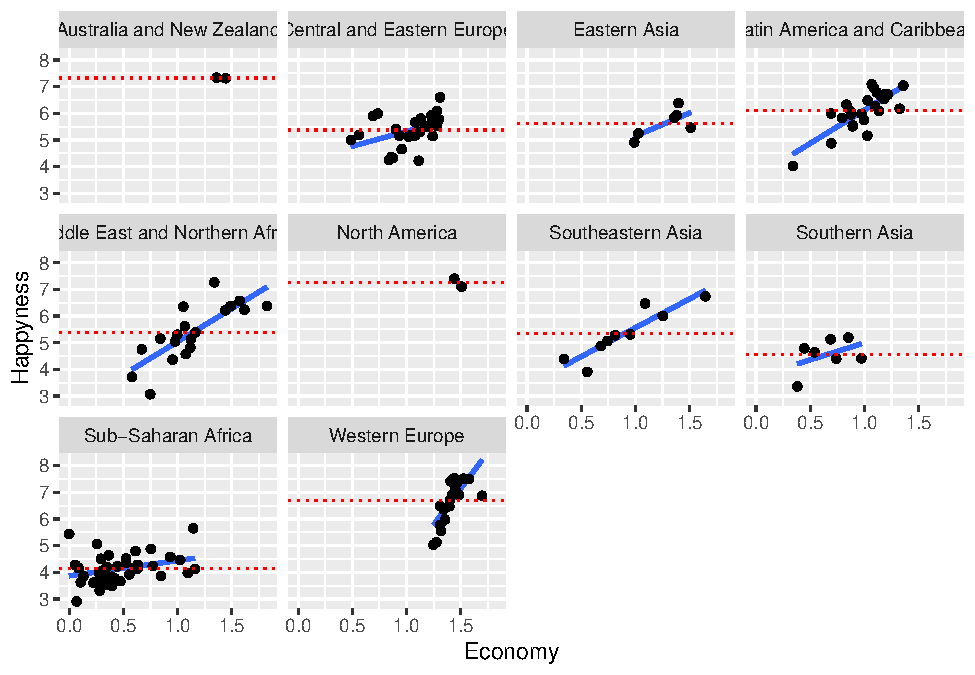
\includegraphics{04-regression_files/figure-latex/unnamed-chunk-4-1.pdf}

Given what we see in the data, we can try two different models:

\begin{Shaded}
\begin{Highlighting}[]
\FunctionTok{library}\NormalTok{(lme4)}
\CommentTok{\#\textgreater{} Loading required package: Matrix}
\CommentTok{\#\textgreater{} }
\CommentTok{\#\textgreater{} Attaching package: \textquotesingle{}Matrix\textquotesingle{}}
\CommentTok{\#\textgreater{} The following objects are masked from \textquotesingle{}package:tidyr\textquotesingle{}:}
\CommentTok{\#\textgreater{} }
\CommentTok{\#\textgreater{}     expand, pack, unpack}
\NormalTok{happy.mixed.model }\OtherTok{\textless{}{-}}  \FunctionTok{lmer}\NormalTok{(Happiness.Score }\SpecialCharTok{\textasciitilde{}}\NormalTok{ Economy..GDP.per.Capita. }\SpecialCharTok{+}\NormalTok{ Health..Life.Expectancy.}\SpecialCharTok{+}\NormalTok{ Generosity }\SpecialCharTok{+}\NormalTok{ (}\DecValTok{1}\SpecialCharTok{|}\NormalTok{Region), }\AttributeTok{data =}\NormalTok{ happiness\_2016)}

\FunctionTok{summary}\NormalTok{(happy.mixed.model)}
\CommentTok{\#\textgreater{} Linear mixed model fit by REML [\textquotesingle{}lmerMod\textquotesingle{}]}
\CommentTok{\#\textgreater{} Formula: }
\CommentTok{\#\textgreater{} Happiness.Score \textasciitilde{} Economy..GDP.per.Capita. + Health..Life.Expectancy. +  }
\CommentTok{\#\textgreater{}     Generosity + (1 | Region)}
\CommentTok{\#\textgreater{}    Data: happiness\_2016}
\CommentTok{\#\textgreater{} }
\CommentTok{\#\textgreater{} REML criterion at convergence: 288.4}
\CommentTok{\#\textgreater{} }
\CommentTok{\#\textgreater{} Scaled residuals: }
\CommentTok{\#\textgreater{}     Min      1Q  Median      3Q     Max }
\CommentTok{\#\textgreater{} {-}3.7228 {-}0.5314  0.0542  0.6596  3.6518 }
\CommentTok{\#\textgreater{} }
\CommentTok{\#\textgreater{} Random effects:}
\CommentTok{\#\textgreater{}  Groups   Name        Variance Std.Dev.}
\CommentTok{\#\textgreater{}  Region   (Intercept) 0.1295   0.3599  }
\CommentTok{\#\textgreater{}  Residual             0.3302   0.5746  }
\CommentTok{\#\textgreater{} Number of obs: 157, groups:  Region, 10}
\CommentTok{\#\textgreater{} }
\CommentTok{\#\textgreater{} Fixed effects:}
\CommentTok{\#\textgreater{}                          Estimate Std. Error t value}
\CommentTok{\#\textgreater{} (Intercept)                3.0080     0.2890  10.407}
\CommentTok{\#\textgreater{} Economy..GDP.per.Capita.   1.5252     0.2136   7.142}
\CommentTok{\#\textgreater{} Health..Life.Expectancy.   1.1030     0.4661   2.367}
\CommentTok{\#\textgreater{} Generosity                 1.2551     0.4088   3.070}
\CommentTok{\#\textgreater{} }
\CommentTok{\#\textgreater{} Correlation of Fixed Effects:}
\CommentTok{\#\textgreater{}             (Intr) E..GDP H..L.E}
\CommentTok{\#\textgreater{} Ec..GDP..C. {-}0.217              }
\CommentTok{\#\textgreater{} Hlth..Lf.E. {-}0.468 {-}0.624       }
\CommentTok{\#\textgreater{} Generosity  {-}0.415  0.174 {-}0.118}

\NormalTok{happy.mixed.model}\FloatTok{.2} \OtherTok{\textless{}{-}}  \FunctionTok{lmer}\NormalTok{(Happiness.Score }\SpecialCharTok{\textasciitilde{}}\NormalTok{ Economy..GDP.per.Capita. }\SpecialCharTok{+}\NormalTok{ Health..Life.Expectancy.}\SpecialCharTok{+}\NormalTok{ Generosity }\SpecialCharTok{+}\NormalTok{ (Economy..GDP.per.Capita.}\SpecialCharTok{|}\NormalTok{Region), }
                             \AttributeTok{data =}\NormalTok{ happiness\_2016)}

\FunctionTok{summary}\NormalTok{(happy.mixed.model)}
\CommentTok{\#\textgreater{} Linear mixed model fit by REML [\textquotesingle{}lmerMod\textquotesingle{}]}
\CommentTok{\#\textgreater{} Formula: }
\CommentTok{\#\textgreater{} Happiness.Score \textasciitilde{} Economy..GDP.per.Capita. + Health..Life.Expectancy. +  }
\CommentTok{\#\textgreater{}     Generosity + (1 | Region)}
\CommentTok{\#\textgreater{}    Data: happiness\_2016}
\CommentTok{\#\textgreater{} }
\CommentTok{\#\textgreater{} REML criterion at convergence: 288.4}
\CommentTok{\#\textgreater{} }
\CommentTok{\#\textgreater{} Scaled residuals: }
\CommentTok{\#\textgreater{}     Min      1Q  Median      3Q     Max }
\CommentTok{\#\textgreater{} {-}3.7228 {-}0.5314  0.0542  0.6596  3.6518 }
\CommentTok{\#\textgreater{} }
\CommentTok{\#\textgreater{} Random effects:}
\CommentTok{\#\textgreater{}  Groups   Name        Variance Std.Dev.}
\CommentTok{\#\textgreater{}  Region   (Intercept) 0.1295   0.3599  }
\CommentTok{\#\textgreater{}  Residual             0.3302   0.5746  }
\CommentTok{\#\textgreater{} Number of obs: 157, groups:  Region, 10}
\CommentTok{\#\textgreater{} }
\CommentTok{\#\textgreater{} Fixed effects:}
\CommentTok{\#\textgreater{}                          Estimate Std. Error t value}
\CommentTok{\#\textgreater{} (Intercept)                3.0080     0.2890  10.407}
\CommentTok{\#\textgreater{} Economy..GDP.per.Capita.   1.5252     0.2136   7.142}
\CommentTok{\#\textgreater{} Health..Life.Expectancy.   1.1030     0.4661   2.367}
\CommentTok{\#\textgreater{} Generosity                 1.2551     0.4088   3.070}
\CommentTok{\#\textgreater{} }
\CommentTok{\#\textgreater{} Correlation of Fixed Effects:}
\CommentTok{\#\textgreater{}             (Intr) E..GDP H..L.E}
\CommentTok{\#\textgreater{} Ec..GDP..C. {-}0.217              }
\CommentTok{\#\textgreater{} Hlth..Lf.E. {-}0.468 {-}0.624       }
\CommentTok{\#\textgreater{} Generosity  {-}0.415  0.174 {-}0.118}
\FunctionTok{summary}\NormalTok{(happy.mixed.model}\FloatTok{.2}\NormalTok{)}
\CommentTok{\#\textgreater{} Linear mixed model fit by REML [\textquotesingle{}lmerMod\textquotesingle{}]}
\CommentTok{\#\textgreater{} Formula: }
\CommentTok{\#\textgreater{} Happiness.Score \textasciitilde{} Economy..GDP.per.Capita. + Health..Life.Expectancy. +  }
\CommentTok{\#\textgreater{}     Generosity + (Economy..GDP.per.Capita. | Region)}
\CommentTok{\#\textgreater{}    Data: happiness\_2016}
\CommentTok{\#\textgreater{} }
\CommentTok{\#\textgreater{} REML criterion at convergence: 276.9}
\CommentTok{\#\textgreater{} }
\CommentTok{\#\textgreater{} Scaled residuals: }
\CommentTok{\#\textgreater{}     Min      1Q  Median      3Q     Max }
\CommentTok{\#\textgreater{} {-}3.7297 {-}0.5007  0.0021  0.6491  3.1793 }
\CommentTok{\#\textgreater{} }
\CommentTok{\#\textgreater{} Random effects:}
\CommentTok{\#\textgreater{}  Groups   Name                     Variance Std.Dev. Corr }
\CommentTok{\#\textgreater{}  Region   (Intercept)              0.09681  0.3111        }
\CommentTok{\#\textgreater{}           Economy..GDP.per.Capita. 0.42078  0.6487   {-}0.87}
\CommentTok{\#\textgreater{}  Residual                          0.29387  0.5421        }
\CommentTok{\#\textgreater{} Number of obs: 157, groups:  Region, 10}
\CommentTok{\#\textgreater{} }
\CommentTok{\#\textgreater{} Fixed effects:}
\CommentTok{\#\textgreater{}                          Estimate Std. Error t value}
\CommentTok{\#\textgreater{} (Intercept)                2.9115     0.2270  12.824}
\CommentTok{\#\textgreater{} Economy..GDP.per.Capita.   1.8639     0.3101   6.010}
\CommentTok{\#\textgreater{} Health..Life.Expectancy.   0.6234     0.4415   1.412}
\CommentTok{\#\textgreater{} Generosity                 1.0923     0.3895   2.805}
\CommentTok{\#\textgreater{} }
\CommentTok{\#\textgreater{} Correlation of Fixed Effects:}
\CommentTok{\#\textgreater{}             (Intr) E..GDP H..L.E}
\CommentTok{\#\textgreater{} Ec..GDP..C. {-}0.390              }
\CommentTok{\#\textgreater{} Hlth..Lf.E. {-}0.323 {-}0.559       }
\CommentTok{\#\textgreater{} Generosity  {-}0.440  0.049 {-}0.092}
\end{Highlighting}
\end{Shaded}

We do not have p-values here hummm!

\begin{Shaded}
\begin{Highlighting}[]
\FunctionTok{library}\NormalTok{(lmerTest)}
\CommentTok{\#\textgreater{} }
\CommentTok{\#\textgreater{} Attaching package: \textquotesingle{}lmerTest\textquotesingle{}}
\CommentTok{\#\textgreater{} The following object is masked from \textquotesingle{}package:lme4\textquotesingle{}:}
\CommentTok{\#\textgreater{} }
\CommentTok{\#\textgreater{}     lmer}
\CommentTok{\#\textgreater{} The following object is masked from \textquotesingle{}package:stats\textquotesingle{}:}
\CommentTok{\#\textgreater{} }
\CommentTok{\#\textgreater{}     step}
\CommentTok{\# Test significance of random effects}
\FunctionTok{ranova}\NormalTok{(happy.mixed.model}\FloatTok{.2}\NormalTok{)}
\CommentTok{\#\textgreater{} ANOVA{-}like table for random{-}effects: Single term deletions}
\CommentTok{\#\textgreater{} }
\CommentTok{\#\textgreater{} Model:}
\CommentTok{\#\textgreater{} Happiness.Score \textasciitilde{} Economy..GDP.per.Capita. + Health..Life.Expectancy. + Generosity + (Economy..GDP.per.Capita. | Region)}
\CommentTok{\#\textgreater{}                                                                 npar}
\CommentTok{\#\textgreater{} \textless{}none\textgreater{}                                                             8}
\CommentTok{\#\textgreater{} Economy..GDP.per.Capita. in (Economy..GDP.per.Capita. | Region)    6}
\CommentTok{\#\textgreater{}                                                                  logLik}
\CommentTok{\#\textgreater{} \textless{}none\textgreater{}                                                          {-}138.45}
\CommentTok{\#\textgreater{} Economy..GDP.per.Capita. in (Economy..GDP.per.Capita. | Region) {-}144.21}
\CommentTok{\#\textgreater{}                                                                    AIC}
\CommentTok{\#\textgreater{} \textless{}none\textgreater{}                                                          292.89}
\CommentTok{\#\textgreater{} Economy..GDP.per.Capita. in (Economy..GDP.per.Capita. | Region) 300.42}
\CommentTok{\#\textgreater{}                                                                    LRT}
\CommentTok{\#\textgreater{} \textless{}none\textgreater{}                                                                }
\CommentTok{\#\textgreater{} Economy..GDP.per.Capita. in (Economy..GDP.per.Capita. | Region) 11.529}
\CommentTok{\#\textgreater{}                                                                 Df}
\CommentTok{\#\textgreater{} \textless{}none\textgreater{}                                                            }
\CommentTok{\#\textgreater{} Economy..GDP.per.Capita. in (Economy..GDP.per.Capita. | Region)  2}
\CommentTok{\#\textgreater{}                                                                 Pr(\textgreater{}Chisq)}
\CommentTok{\#\textgreater{} \textless{}none\textgreater{}                                                                    }
\CommentTok{\#\textgreater{} Economy..GDP.per.Capita. in (Economy..GDP.per.Capita. | Region)   0.003137}
\CommentTok{\#\textgreater{}                                                                   }
\CommentTok{\#\textgreater{} \textless{}none\textgreater{}                                                            }
\CommentTok{\#\textgreater{} Economy..GDP.per.Capita. in (Economy..GDP.per.Capita. | Region) **}
\CommentTok{\#\textgreater{} {-}{-}{-}}
\CommentTok{\#\textgreater{} Signif. codes:  }
\CommentTok{\#\textgreater{} 0 \textquotesingle{}***\textquotesingle{} 0.001 \textquotesingle{}**\textquotesingle{} 0.01 \textquotesingle{}*\textquotesingle{} 0.05 \textquotesingle{}.\textquotesingle{} 0.1 \textquotesingle{} \textquotesingle{} 1}

\CommentTok{\#Test significance of fixed effects}
\NormalTok{ml.happy.mixed.model }\OtherTok{\textless{}{-}} \FunctionTok{update}\NormalTok{(happy.mixed.model, }\AttributeTok{REML =} \ConstantTok{FALSE}\NormalTok{) }\CommentTok{\# this changes the algorithm used to fit the model}

\CommentTok{\#Finally we can test significance}
\FunctionTok{anova}\NormalTok{(}\FunctionTok{as\_lmerModLmerTest}\NormalTok{(ml.happy.mixed.model))}
\CommentTok{\#\textgreater{} Type III Analysis of Variance Table with Satterthwaite\textquotesingle{}s method}
\CommentTok{\#\textgreater{}                           Sum Sq Mean Sq NumDF  DenDF}
\CommentTok{\#\textgreater{} Economy..GDP.per.Capita. 16.9971 16.9971     1 152.49}
\CommentTok{\#\textgreater{} Health..Life.Expectancy.  1.9558  1.9558     1 138.78}
\CommentTok{\#\textgreater{} Generosity                3.1992  3.1992     1 151.95}
\CommentTok{\#\textgreater{}                          F value    Pr(\textgreater{}F)    }
\CommentTok{\#\textgreater{} Economy..GDP.per.Capita. 52.3454 2.119e{-}11 ***}
\CommentTok{\#\textgreater{} Health..Life.Expectancy.  6.0233  0.015356 *  }
\CommentTok{\#\textgreater{} Generosity                9.8524  0.002038 ** }
\CommentTok{\#\textgreater{} {-}{-}{-}}
\CommentTok{\#\textgreater{} Signif. codes:  }
\CommentTok{\#\textgreater{} 0 \textquotesingle{}***\textquotesingle{} 0.001 \textquotesingle{}**\textquotesingle{} 0.01 \textquotesingle{}*\textquotesingle{} 0.05 \textquotesingle{}.\textquotesingle{} 0.1 \textquotesingle{} \textquotesingle{} 1}
\end{Highlighting}
\end{Shaded}

\hypertarget{ploting-the-data-in-a-map}{%
\subsection{Ploting the data in a map}\label{ploting-the-data-in-a-map}}

\begin{Shaded}
\begin{Highlighting}[]
\FunctionTok{require}\NormalTok{(rnaturalearth)}
\CommentTok{\#\textgreater{} Loading required package: rnaturalearth}
\FunctionTok{require}\NormalTok{(rnaturalearthdata)}
\CommentTok{\#\textgreater{} Loading required package: rnaturalearthdata}
\NormalTok{world }\OtherTok{\textless{}{-}} \FunctionTok{ne\_countries}\NormalTok{(}\AttributeTok{scale =} \StringTok{"medium"}\NormalTok{, }\AttributeTok{returnclass =} \StringTok{"sf"}\NormalTok{) }\CommentTok{\# this is another function to get polygons of countries. }
\end{Highlighting}
\end{Shaded}

\begin{Shaded}
\begin{Highlighting}[]
\FunctionTok{library}\NormalTok{(ggplot2)}
\FunctionTok{ggplot}\NormalTok{(}\AttributeTok{data =}\NormalTok{ world) }\SpecialCharTok{+}
    \FunctionTok{theme\_bw}\NormalTok{()}\SpecialCharTok{+} 
    \FunctionTok{geom\_sf}\NormalTok{() }\SpecialCharTok{+} 
    \FunctionTok{xlab}\NormalTok{(}\StringTok{"Longitude"}\NormalTok{) }\SpecialCharTok{+} \FunctionTok{ylab}\NormalTok{(}\StringTok{"Latitude"}\NormalTok{) }\SpecialCharTok{+} 
    \FunctionTok{ggtitle}\NormalTok{(}\StringTok{"World map"}\NormalTok{, }\AttributeTok{subtitle =} \FunctionTok{paste0}\NormalTok{(}\StringTok{"("}\NormalTok{, }\FunctionTok{dim}\NormalTok{(world)[}\DecValTok{1}\NormalTok{], }\StringTok{" countries)"}\NormalTok{))}
\end{Highlighting}
\end{Shaded}

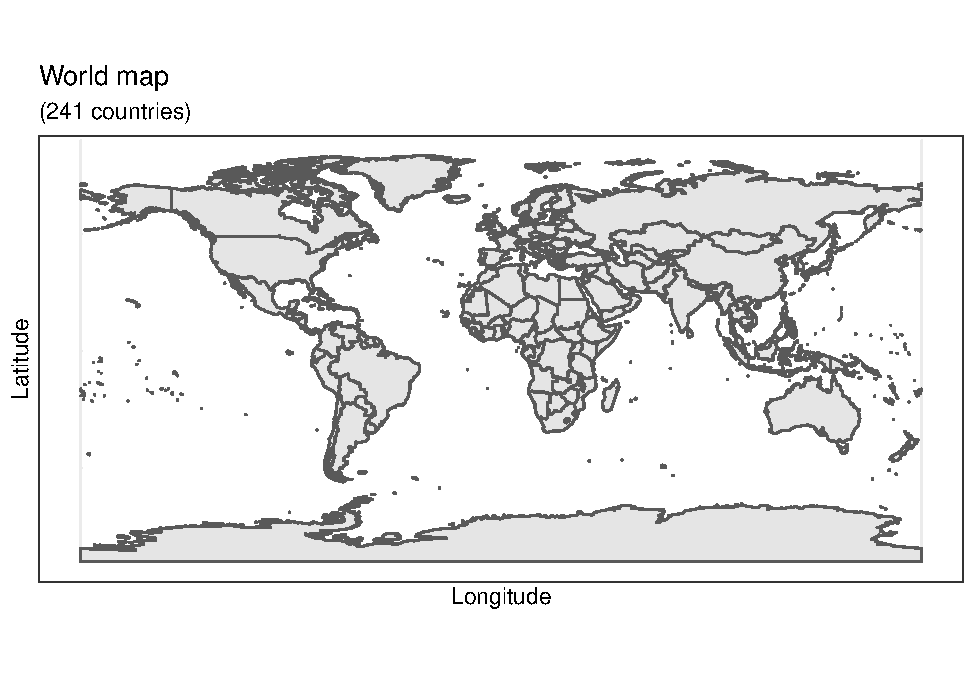
\includegraphics{04-regression_files/figure-latex/unnamed-chunk-8-1.pdf}

\begin{verbatim}
#both df woth the same name of the varaible we will use to join
colnames(happiness_2016)[1] <- "name"
Happiness_GEO <- left_join(world, happiness_2016, by="name")
\end{verbatim}

\begin{verbatim}
ggplot(data = Happiness_GEO) +
    geom_sf(aes(fill = Happiness.Score )) +
    scale_fill_viridis_c(option = "plasma") +  # this allows you to choose different colour scale
    ggtitle("World Happiness Studies")
\end{verbatim}

\hypertarget{where-is-the-model-working-better}{%
\subsubsection{Where is the model working better?}\label{where-is-the-model-working-better}}

\begin{verbatim}
happy.predictions <- predict(happy.mixed.model)
#Expected - Observed
happy.residuasl <-  (happiness_2016$Happiness.Score - happy.predictions) # Obaserved - predicted
Happiness_2016$Model.Residuals <- happy.residuasl
Happiness_GEO <- left_join(world, Happiness_2016, by="name")
\end{verbatim}

\begin{verbatim}
ggplot(data = Happiness_GEO) +
    geom_sf(aes(fill = Model.Residuals )) +
    scale_fill_viridis_c(option = "plasma") +  # this allows you to choose different colour scale
    ggtitle("World Happiness Studies")
\end{verbatim}

\hypertarget{blocks}{%
\chapter{Blocks}\label{blocks}}

\hypertarget{equations}{%
\section{Equations}\label{equations}}

Here is an equation.

\begin{equation} 
  f\left(k\right) = \binom{n}{k} p^k\left(1-p\right)^{n-k}
  \label{eq:binom}
\end{equation}

You may refer to using \texttt{\textbackslash{}@ref(eq:binom)}, like see Equation \eqref{eq:binom}.

\hypertarget{theorems-and-proofs}{%
\section{Theorems and proofs}\label{theorems-and-proofs}}

Labeled theorems can be referenced in text using \texttt{\textbackslash{}@ref(thm:tri)}, for example, check out this smart theorem \ref{thm:tri}.

\begin{theorem}
\protect\hypertarget{thm:tri}{}\label{thm:tri}For a right triangle, if \(c\) denotes the \emph{length} of the hypotenuse
and \(a\) and \(b\) denote the lengths of the \textbf{other} two sides, we have
\[a^2 + b^2 = c^2\]
\end{theorem}

Read more here \url{https://bookdown.org/yihui/bookdown/markdown-extensions-by-bookdown.html}.

\hypertarget{callout-blocks}{%
\section{Callout blocks}\label{callout-blocks}}

The \texttt{bs4\_book} theme also includes special callout blocks, like this \texttt{.rmdnote}.

You can use \textbf{markdown} inside a block.

\begin{Shaded}
\begin{Highlighting}[]
\FunctionTok{head}\NormalTok{(beaver1, }\AttributeTok{n =} \DecValTok{5}\NormalTok{)}
\CommentTok{\#\textgreater{}   day time  temp activ}
\CommentTok{\#\textgreater{} 1 346  840 36.33     0}
\CommentTok{\#\textgreater{} 2 346  850 36.34     0}
\CommentTok{\#\textgreater{} 3 346  900 36.35     0}
\CommentTok{\#\textgreater{} 4 346  910 36.42     0}
\CommentTok{\#\textgreater{} 5 346  920 36.55     0}
\end{Highlighting}
\end{Shaded}

It is up to the user to define the appearance of these blocks for LaTeX output.

You may also use: \texttt{.rmdcaution}, \texttt{.rmdimportant}, \texttt{.rmdtip}, or \texttt{.rmdwarning} as the block name.

The R Markdown Cookbook provides more help on how to use custom blocks to design your own callouts: \url{https://bookdown.org/yihui/rmarkdown-cookbook/custom-blocks.html}

\hypertarget{sharing-your-book}{%
\chapter{Sharing your book}\label{sharing-your-book}}

\hypertarget{publishing}{%
\section{Publishing}\label{publishing}}

HTML books can be published online, see: \url{https://bookdown.org/yihui/bookdown/publishing.html}

\hypertarget{pages}{%
\section{404 pages}\label{pages}}

By default, users will be directed to a 404 page if they try to access a webpage that cannot be found. If you'd like to customize your 404 page instead of using the default, you may add either a \texttt{\_404.Rmd} or \texttt{\_404.md} file to your project root and use code and/or Markdown syntax.

\hypertarget{metadata-for-sharing}{%
\section{Metadata for sharing}\label{metadata-for-sharing}}

Bookdown HTML books will provide HTML metadata for social sharing on platforms like Twitter, Facebook, and LinkedIn, using information you provide in the \texttt{index.Rmd} YAML. To setup, set the \texttt{url} for your book and the path to your \texttt{cover-image} file. Your book's \texttt{title} and \texttt{description} are also used.

This \texttt{bs4\_book} provides enhanced metadata for social sharing, so that each chapter shared will have a unique description, auto-generated based on the content.

Specify your book's source repository on GitHub as the \texttt{repo} in the \texttt{\_output.yml} file, which allows users to view each chapter's source file or suggest an edit. Read more about the features of this output format here:

\url{https://pkgs.rstudio.com/bookdown/reference/bs4_book.html}

Or use:

\begin{Shaded}
\begin{Highlighting}[]
\NormalTok{?bookdown}\SpecialCharTok{::}\NormalTok{bs4\_book}
\end{Highlighting}
\end{Shaded}


  \bibliography{book.bib,packages.bib}

\end{document}
